



\chapter{Spin conservation in bicircular high-order harmonic generation}
\label{chap:spin-HHG}
This chapter examines high-order harmonic generation from the perspective of looking for harmonics with circular polarization, which is technologically interesting and also provides a window into the structure of the conservation laws in HHG. In particular, we examine the first experimental scheme to successfully produce circularly polarized harmonics, using a combination of two drivers, one at $\SI{800}{nm}$ and its second harmonic at $\SI{400}{nm}$, with opposite circular polarizations (`bicircular' fields), and we describe a photon-picture model for the exchange of spin angular momentum in the process.





This chapter contains work previously published in references

\begin{enumerate}
\item[{\hypersetup{citecolor=black}\citealp{Ivanov_nature_photonics_2014}}.]
\textsc{M.~Ivanov and E.~Pisanty}.
\newblock High-harmonic generation:\ taking control of polarization.
\newblock \href{http://dx.doi.org/10.1038/nphoton.2014.141}{
          \emph{Nature Photon.} \textbf{8} no.~7, pp.~501--503 (2014)} (News \& Views).

\item[{\hypersetup{citecolor=black}\citealp{Pisanty_spin_conservation_2014}}.]
\textsc{E.~Pisanty, S.~Sukiasyan and M.~Ivanov}.
\newblock Spin conservation in high-order-harmonic generation using bicircular fields. 
\newblock \href{http://dx.doi.org/10.1103/PhysRevA.90.043829}{
          \emph{Phys. Rev. A} \textbf{90} no.~4, p. 043\,829 (2014)}.
\newblock \href{http://arxiv.org/abs/1404.6242}{{arXiv}:1404.6242}.

\end{enumerate}





\section{Circular polarization in high-order harmonic generation}
\label{sec:circular-harmonics-intro}
As we saw in chapter~\ref{chap:HHG-intro}, HHG is a very versatile process and it is very useful both as a tool to explore the dynamics and structure of atoms and molecules using the harmonic generation process itself, as well as a flexible source of short, bright, coherent pulses of high-frequency radiation for use in further experiments. Over the two decades since the discovery of HHG, significant progress has been made in improving the toolset that it provides as a light source, by increasing the cut-off frequency, flux and coherence, the design of gating schemes that allow the use of a single radiation burst, and the increasing control over the emitted radiation, among many others.

One tool that has mostly lacked from this development is the polarization of the emitted harmonics, which has been essentially confined to linear polarizations along the polarization of the driving IR field. This allows for plenty of interesting physics, including vector manipulations on light by using multiple pulses with different linear polarizations, but it also rules out circularly polarized pulses, which limits the extent to which the angular momentum structure of atoms and molecules can be probed.

More importantly, however, the lack of circularly polarized pulses completely eliminates the extent to which the chiral structures of matter can be investigated. This is an important consideration in the study of biomolecules, most of which are chiral~\cite{hergenhahn_pecd-camphor-x-ray_2004, bowering_x-ray-molecular-dichroism_2001}, as well as in the study of magnetic properties of matter~\cite{ boeglin_synchrotron-circular_2010, stamm_femtosecond-xmcd_2007}, since the magnetization of a material is also a chiral property. In fact, the X-ray magnetic circular dichroism (XMCD) of magnetic materials -- the differential absorption of one circular polarization over its opposite handedness by a magnetized material -- is an important tool in their study.


Fortunately, it has been possible for some time to produce the circularly polarized radiation required by these fields, using synchrotron and free-electron laser (FEL) radiation produced using suitable undulators~\cite{bahrdt_fel-circular-initial_1992, allaria_FEL-circular_2014, lutman_FEL-polarization_2016}, and among other things this has enabled the growth of XMCD as a tool for the time-domain study of fast magnetization processes. However, synchrotrons and FELs are facility experiments, requiring a large and particle accelerator to function, and this makes beam time on those experiments a scarce resource. Generally, this is solved by going to table-top sources based on HHG, but for circular polarizations this is an issue; it is therefore desirable to extend the capabilities of HHG to include chiral polarizations with nonzero helicity.



The immediate response to this problem, of course, is to try to produce high-order harmonics using an elliptically polarized driver, but this does not work. The generation of high-order harmonics is in its essence a recollision-based phenomenon, and in the presence of an elliptical driver the three-step-model electrons will be shifted aside and miss the ion in their oscillations, quickly quenching the harmonic emission~\cite{antoine_harmonics-polarization_1997, moller_hhg-elliptical-fields_2012, li_quantum-orbit-ellipticity-hhg_2013}. (Moreover, as we shall see later, there are fundamental selection rules~\cite{SelectionRulesInHHG, averbukh_stability_2002} which prevent a circularly polarized driver from emitting \textit{any} harmonic radiation.)


Similarly, it is tempting to attempt to borrow from the optical domain techniques and look for an extreme-ultraviolet (XUV) waveplate to apply to linearly-polarized HHG pulses. Unfortunately, there are no transmissive waveplates in the XUV regime, as materials become opaque at the thicknesses where they would become birefringent. It is possible to build circular polarizers using a succession of grazing-incidence reflections~\cite{vodungbo_hhg-waveplate_2011}, but this is a challenging technique and it has not gained much traction~\cite{willems_hhg-waveplate_2015}. Moreover, the efficiency of such polarizers is very low, limiting the source brightness and therefore the usefulness for applications; this circular HHG signal can be amplified using a plasma soft-X-ray-laser amplifier~ \cite{depresseux_hhg-then-plasma-laser_2015}, but this raises the experiment's complexity even further.



Over the years there have also been several proposals for how to provide for circularly-polarized HHG, generally challenging to implement; these have included 
%
the use of multi-colour beams, with orthogonal polarizations~\cite{ruiz_elliptical-pulses-two-color_2009} 
%
or propagation directions~\cite{tong-chu_crossed-beam_1998, fleischer_linear-plus-elliptical-driver_2013}, 
%
the use of strong static~\cite{borca_static-field-circular-harmonics_2000}
%
and terahertz~\cite{yuan_elliptical-terahertz_2013} fields,
%
nanostructure arrays~\cite{husakou_circular-harmonics-nanostructures_2011}, 
%
and quasi phase matching with a birefringent waveguide~\cite{liu_circular-hhg-quasi-phase-matching_2012}. 



Somewhat more happily, circular harmonics have been produced using a single linearly-polarized driver on aligned molecules~\cite{zhou_aligned-molecules-elliptical-hhg_2009, mairesse_high-harmonic-spectroscopy_2010}, though at very low ellipticity and efficiency, 
%
as well as with or\-tho\-go\-na\-lly-polarized two-colour drivers~\cite{lambert_circular-hhg-cross-polarized_2015, stremoukhov_elliptical-harmonics_2016}
%
and, at low efficiency, with atoms and elliptically polarized drivers~\cite{ weihe_harmonics-polarization_1995, antoine_harmonics-polarization_1997, strelkov_harmonics-polarization-origin_2011}
%
More recently, and more promisingly, Ferré et al. used an elliptical driver, with resonantly produced harmonics, to produce reasonably bright elliptically polarized high-order harmonics~\cite{ferre_circular-harmonics_2015}.

The real breakthrough, however, came in 2014, when A.\,Fleischer and co-workers produced bright, fully circular high-order harmonics using only three-step-model physics~\cite{fleischer_spin_2014}. They used two counter-rotating circularly polarized drivers of equal intensity but different frequency, one at $\SI{800}{nm}$ and its second harmonic at $\SI{400}{nm}$, which combine to make the trefoil-shaped field shown in \reffig{f8-bicircular-field-sketch}, and which is known in the literature as a `bicircular' configuration. This field shape then permits recollisions, and its selection rules permit harmonic emission at arbitrarily high frequencies. It will be our main object of study in this chapter.


\begin{figure}[htb]
  \centering
  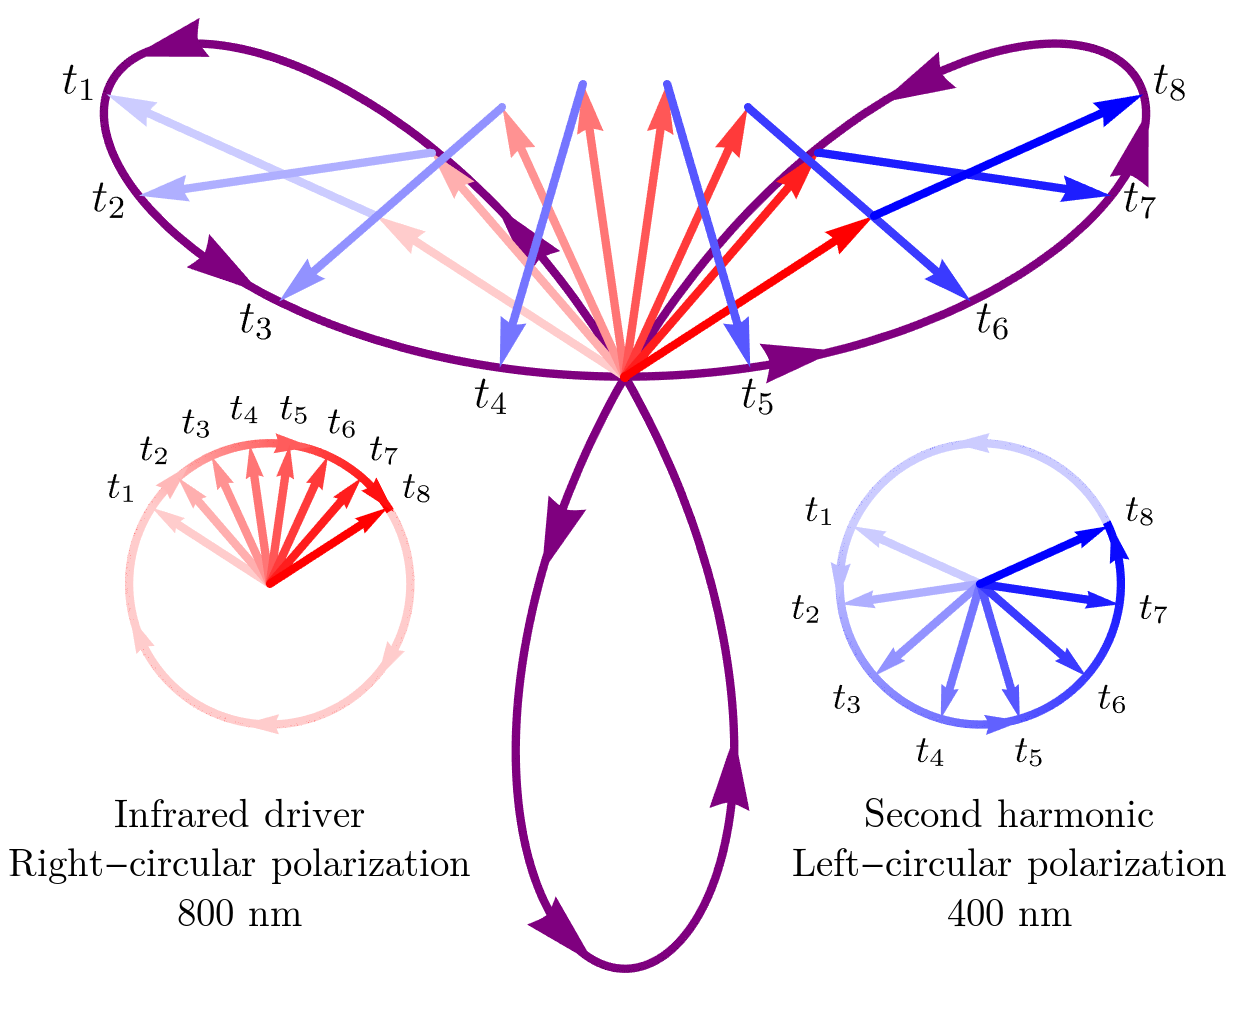
\includegraphics[scale=1]{8-Spin-HHG/Figures/figure8A.png}
  \caption[
  Bicircular field configuration: a right-circular $\SI{800}{nm}$ field combines with a left-circular $\SI{400}{nm}$ one to make a trefoil-shaped total field
  ]{
  Bicircular field configuration, formed by the equal-intensities superposition of an infrared right-circular driver at $\SI{800}{nm}$ (left inset) and its second harmonic at $\SI{400}{nm}$ with left-circular polarization (right inset). Both fields are shown as arrows over a third of the infrared period; in this interval the right-circular infrared covers a \SI{120}{\degree} angle, while the second harmonic covers \SI{240}{\degree} in the opposite direction, so they are equal at the start and end of the interval. When superposed, the two fields combine to form the three-lobed trefoil shown in purple.
  }
  \label{f8-bicircular-field-sketch}
\end{figure}

Bicircular fields had been explored in the literature for some time~\cite{ EichmannExperiment, SFALong, SFAMilosevic, milosevic_bicircular-hhg_2000, SFAMilosevicBecker, milosevic_unusual-nonlinear-polarization_2000, milosevic_hhg-laser-phys_2001, averbukh_stability_2002, SFACeccherini, MilosevicIsolatedPulses}, and indeed an early experiment \cite{EichmannExperiment} implemented the variation, observing signal with the correct selection rules, but (for reasons which remain unclear) it was not followed up experimentally for some time. The recent detection by Fleischer et al., however, sparked a flurry of interest in the mechanism, both theoretical and experimental.


Experimentally, the available information about the process has grown considerably. In their initial detection, Fleischer et al. used a rotating linear polarizer, as shown in \reffig{f8-fleischer-bicircular-spectrum-a}, with a very low dependence of the signal on the polarizer angle, implying that the harmonics were circularly polarized. This was further confirmed when later experiments swapped the gas jet for a gas-filled hollow waveguide, allowing for enough signal to perform X-ray magnetic circular dichroism experiments~\cite{kfir_generation_2015, fan_bright-circularly_2015}, providing an unambiguous confirmation of a nonzero helicity.

(On the other hand, the available XMCD experiments using this XUV source do not quite agree with the corresponding measurements performed on synchrotron light sources, which are more established. This does not invalidate the observation of the \textit{presence} of helicity, since mirror versions of the same observe different results, regardless of their orientation, but it does call for much more careful polarimetry measurements on that radiation to confirm the amount of helicity of the radiation. Unfortunately, reliable XUV polarimetry in this regime, particularly with respect to the helicity of the radiation, is a very challenging task.)


Further experimental developments have expanded the mechanism to other combinations of driver wavelengths~\cite{fan_bright-circularly_2015}, explored the role of chirality in the phase-matching conditions for generation inside a hollow waveguide~\cite{kfir_chiral-phase-matching_2016}, and simplified the non-collinear Mach-Zehnder-type interferometer used in \citer{fleischer_spin_2014} to obtain the bicircular fields, as shown in \reffig{f8-fleischer-bicircular-spectrum-a}, for a simpler in-line configuration~\cite{kfir_in-line-bicircular_2016}. In addition, and of special interest for our following chapter, the bicircular configuration has also been extended to non-collinear beam configurations~\cite{hickstein_non-collinear_2015}, allowing for the spatial selection of beams with different helicities. 

$\quad$


\begin{figure}[b!h]
  \centering
  \subfloat{\label{f8-fleischer-bicircular-spectrum-a}}
  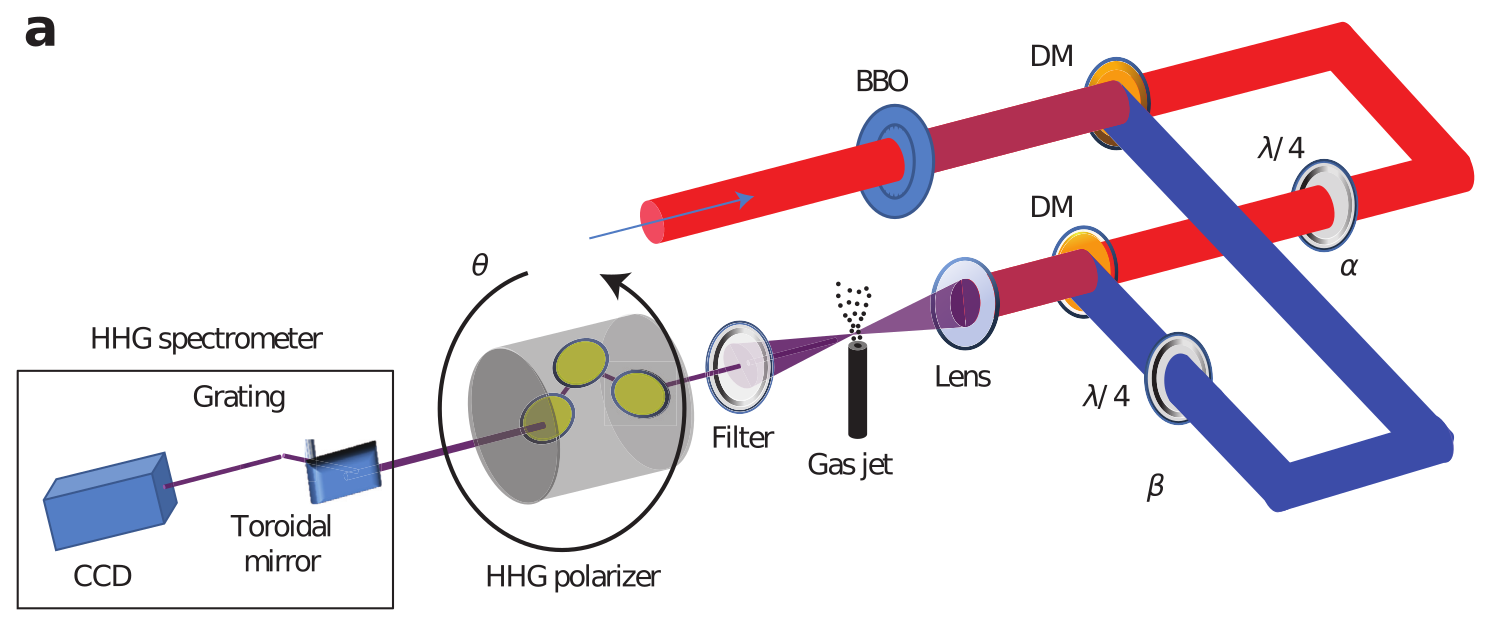
\includegraphics[scale=0.85]{8-Spin-HHG/Figures/figure8Ba.png}
  \\[4mm]
  \subfloat{\label{f8-fleischer-bicircular-spectrum-b}}
  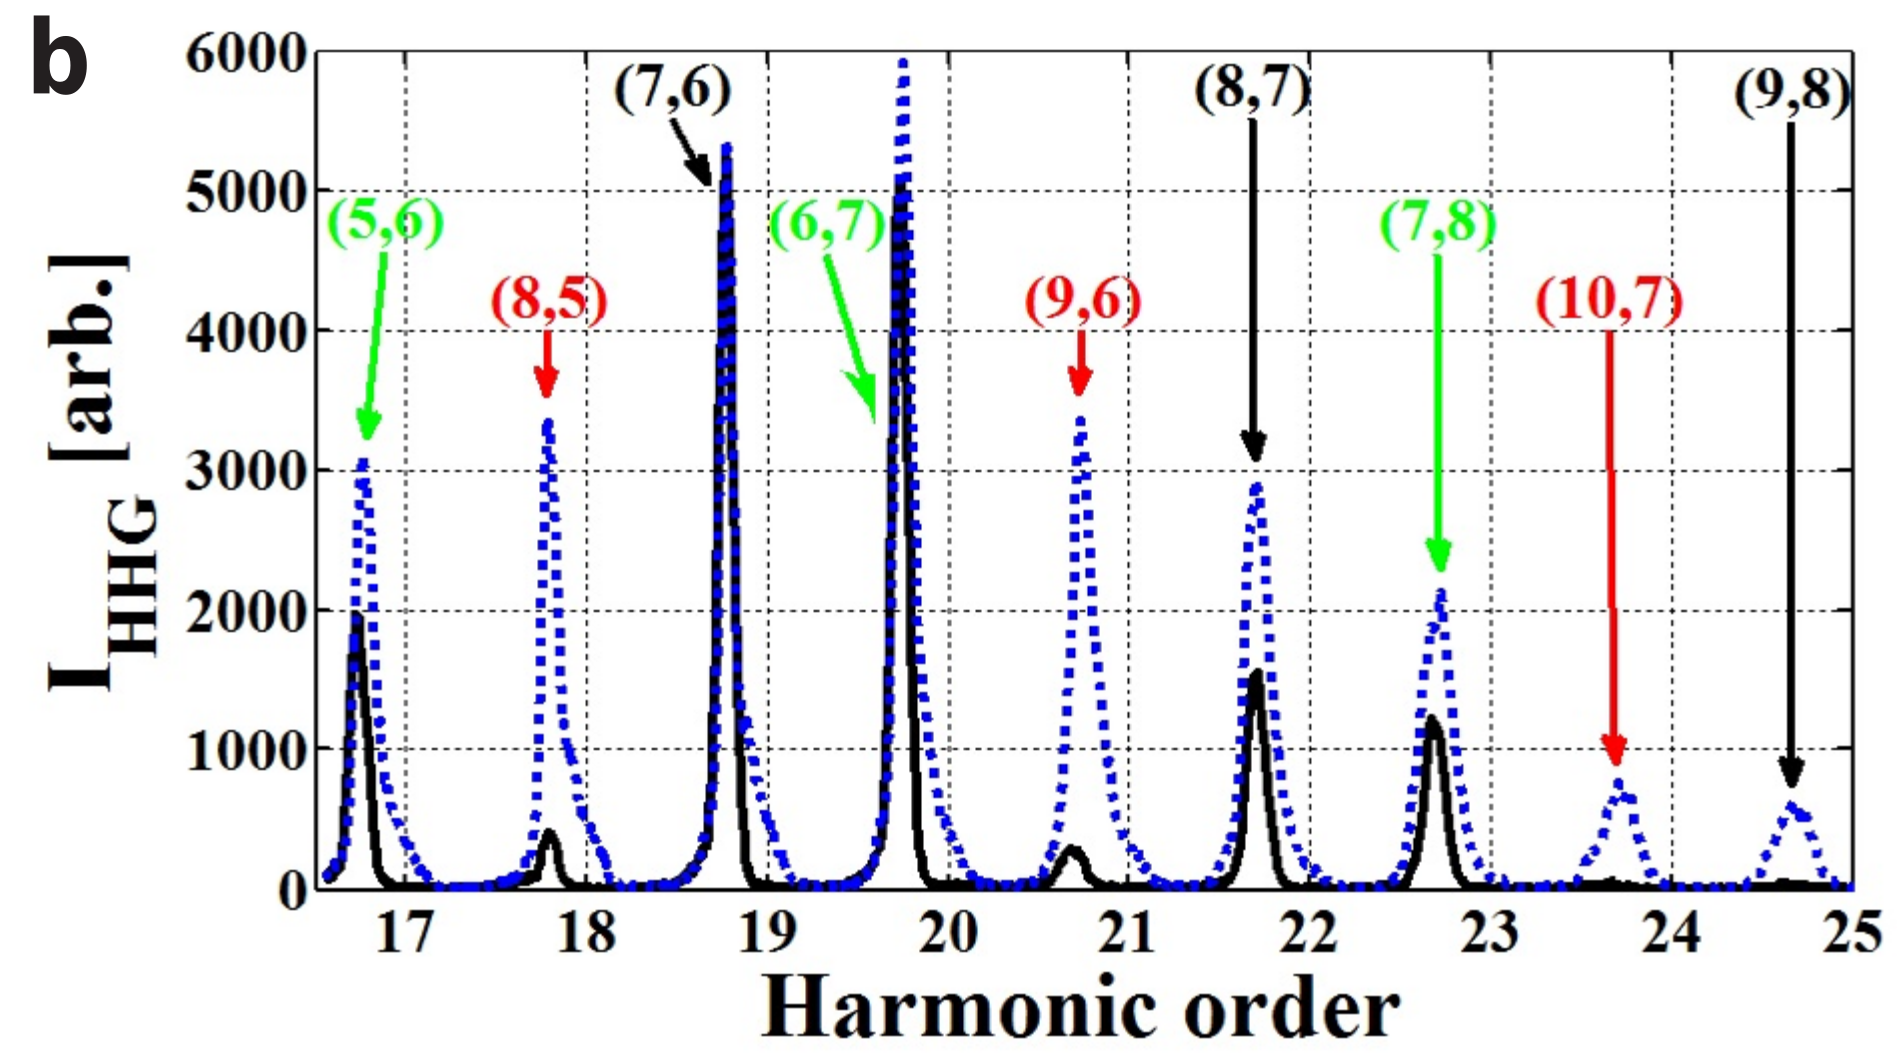
\includegraphics[height=4cm]{8-Spin-HHG/Figures/figure8Bb.png}
  \hspace{5mm}
  \subfloat{\label{f8-fleischer-bicircular-spectrum-c}}
  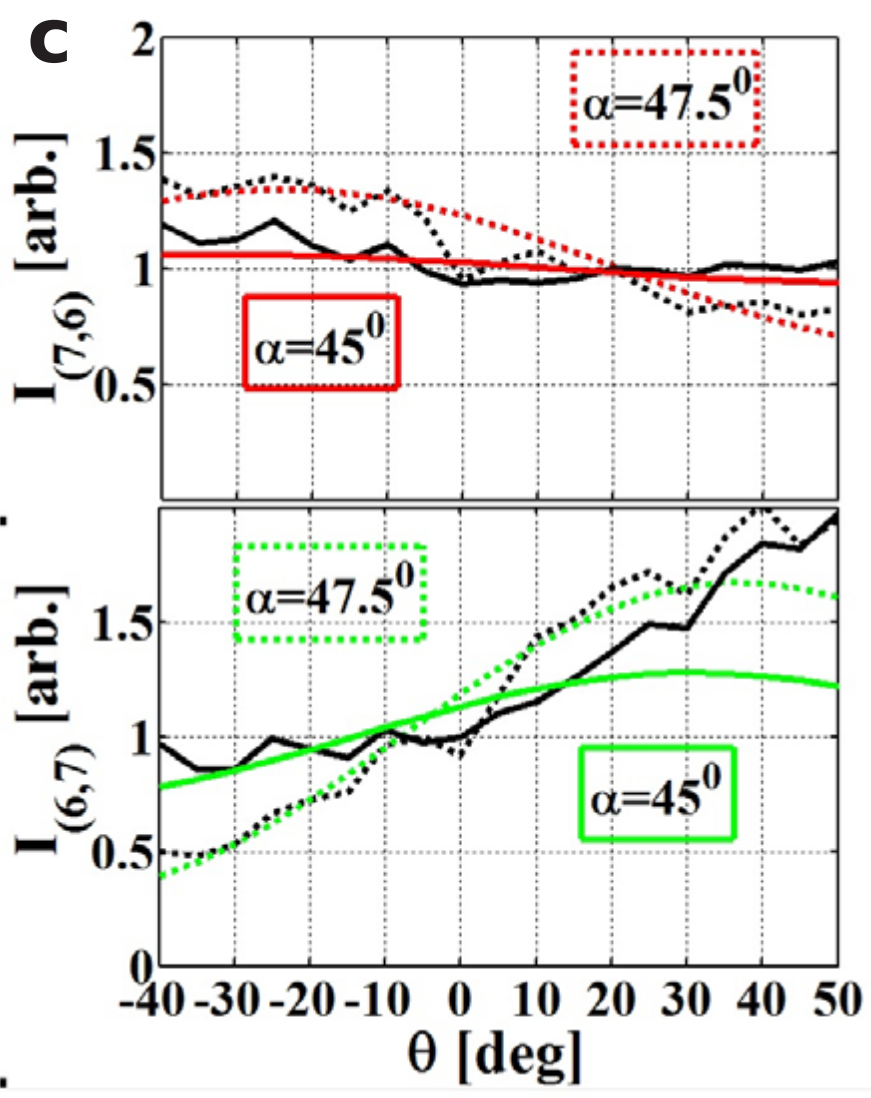
\includegraphics[height=4cm]{8-Spin-HHG/Figures/figure8Bc.png}
  \caption[
  Initial observation of bicircular high-order harmonics by A. Fleischer~et~al.
  ]{
  Initial observation of bicircular high-order harmonics~\cite{fleischer_spin_2014}, showing a schematic of the experiment~\protect\subref{f8-fleischer-bicircular-spectrum-a}, and a sample harmonic spectrum~\protect\subref{f8-fleischer-bicircular-spectrum-b}. The second harmonic is generated in a nonlinear BBO crystal, and the two fields are split and recombined using dichroic mirrors (DM), with their circular polarizations set using independent waveplates. 
  The harmonics are emitted in pairs of lines, at intensities comparable to those with linearly polarized drivers, shown dashed in \protect\subref{f8-fleischer-bicircular-spectrum-b}.
  After the harmonic generation in a gas jet, a rotating linear polarizer tests the polarization of the harmonics, with the corresponding traces (shown in \protect\subref{f8-fleischer-bicircular-spectrum-c}) displaying little variation in the intensity with respect to the polarizer angle.
%  \\ \ \\
  Figure excerpted from \citer{fleischer_spin_2014}.
  }
  \label{f8-fleischer-bicircular-spectrum}
\end{figure}

\copyrightfootnote{
\reffig{f8-fleischer-bicircular-spectrum} copyright tagline.
}

$\quad$

Finally, it is also important to note that recent experiments performing detailed polarimetry on the resultant HHG radiation~\cite{veyrinhas_polarimetry-original_2013, veyrinhas_depolarized-hhg-atto_2015, chen_tomographic-hhg-polarimetry_2016}, with the crucial finding that the harmonics can be produced in a partially depolarized state~\cite{veyrinhas_depolarized-hhg-atto_2015}. The origin of this depolarization is completely unclear, though it may to originate from spatial variations of the harmonic polarization across the laser focus. Regardless of its origin, the finding underscores the need for helicity-dependent XMCD observations, above and beyond the rotational invariance with respect to a linear polarizer, as the hallmark confirmation that circular harmonics are being emitted.



On the theory side, most of the early papers focus on explaining the original observation~\cite{EichmannExperiment} and providing a suitable quantum-orbit SFA theory \cite{SFALong, SFAMilosevicBecker,milosevic_hhg-laser-phys_2001} and understanding the temporal structure of the HHG emission~\cite{milosevic_unusual-nonlinear-polarization_2000}, which we will also explore below. In the aftermath of the initial observation, interest has shifted to the angular momentum structure of the emission [\citealp{Ivanov_nature_photonics_2014, Pisanty_spin_conservation_2014}, with a similar later observation in~\citealp{milosevic_bicircular-angular-momentum_2015}], which is the work we will explore in depth in this chapter, as well as the implications for selection rules for molecules in bicircular fields~\cite{reich-madsen_molecular-symmetries_2016, baykusheva_bicircular-hhg-spectroscopy, liu_selection-rules-hhg_2016, mauger_bicircular-molecular-hhg, odzak_polyatomic-bicircular_2016, yuan-bandrauk_circular-hhg-extended-asymmetric-molecules_2011}, and the search for ways to maximize the global helicity of the harmonic emission~\cite{kfir_chiral-phase-matching_2016, milosevic_elliptical-apt_2015, milosevic_circularly_2015, medisauskas_generating_2016} and to obtain single circularly polarized attosecond pulses~\cite{ medisauskas_generating_2016, hernandez_isolated-circular-pulses_2016}. Finally, to round things out, is a clean analysis of bicircular HHG in a frame that rotates with the total electric field~\cite{reich-madsen_rotating-frame-bicircular_2016}.




In addition to this, because they allow tunnel-ionized electrons to return to the ion where they can interact with it, bicircular fields have also shown to be of considerable interest for studies of strong-field ionization~\cite{ mancuso_bicircular-ionization_2015,mancuso_bicircular-rescattering_2016,ngoko-starace_multistart-spiral-ionization_2016, milosevic_bicircular-ionization-sfa_2016, chaloupka_bicircular-double-ionization_2016}, as well as above-threshold detachment~\cite{kramo_bicircular-atd_2007}, electron rescattering~\cite{hasovic_rescattering-bicircular_2016}, non-sequential double ionization~\cite{eckart_bicircular-nsdi_2016},  and laser-assisted recombination~\cite{odzak_bicircular-laser-assisted-recombination_2015}, as well as for inducing spin polarization for electrons ionized by strong fields in the presence of spin-orbit coupling~\cite{ milosevic_bicircular-spin-polarization_2016, hartung_spin-polarization-ionization_2016}.











\section{Selection rules in bicircular HHG}
\label{sec:hhg-selection-rules}
There are multiple ways to understand the harmonic emission induced by bicircular fields, and much of our analysis will focus on a frequency-domain analysis of the radiation in terms of photon transfers within a parametric optical process. However, it is important to ground this first in a time-dependent view of the induced harmonic dipole.


HHG is, at its core, a recollision phenomenon, and bicircular fields are only able to produce high-order harmonics efficiently because electrons that are tunnel-ionized near the peak of each lobe have a large probability of recolliding with the ion. The trajectories in question are mostly of the  character showin in \reffig{f8-fleischer-trajectories}, with the ionization just before one field maximum and the recollision at the close of the following lobe. 

This has two important consequences. The first is that each burst of XUV emission comes from a single recollision event with a well-defined direction, so each burst of radiation will mostly be linearly polarized. However, because of the three-fold symmetry of the field, each of these recollisions, with their attendant bursts of XUV radiation, is necessarily mirrored by two other identical sets of trajectories and radiation bursts, trailing each other by a third of a period of the fundamental and rotated with respect to each other by~\SI{120}{\degree}. The HHG radiation, then, consists of a train of attosecond pulses, linearly polarized along directions that rotate steadily during the pulse, as shown in \reffig{f8-typical-bicircular-apt}.




%\pagebreak

\begin{figure}[h!]
  
  \vspace{10mm}
  
  \centering
  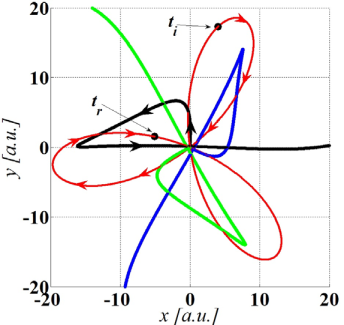
\includegraphics[scale=0.8]{8-Spin-HHG/Figures/figure8D.png}
  \caption[
  Typical trajectories that result in HHG emission from bicircular fields, as calculated by A. Fleischer~et~al.
  ]{
  Typical trajectories resulting in harmonic emission in a bicircular field, with the ionization and recollision times $t_i$ and $t_r$ corresponding to the trajectory shown in black. Because of the symmetry of the field, there will be two additional identical trajectories (shown in blue and green) each period, oriented at \SI{120}{\degree} from each other.
  Figure excerpted from \citer{fleischer_spin_2014}.
  }
  \label{f8-fleischer-trajectories}
  
  \vspace{15mm}
  
  \centering
  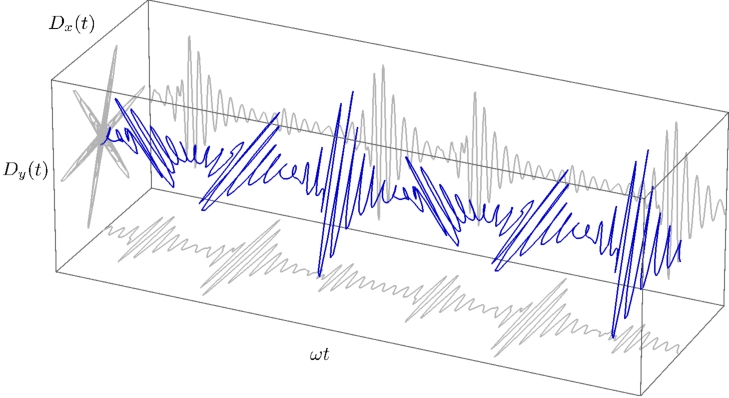
\includegraphics[scale=1]{8-Spin-HHG/Figures/figure8C.pdf}
  \caption[
  Typical attosecond pulse train produced by bicircular fields: a train of linearly polarized attosecond bursts, rotated by $\SI{120}{\degree}$ from each other
  ]{
  Typical attosecond pulse train produced by the bicircular fields of \reffig{f8-bicircular-field-sketch}; the harmonic dipole consists of a train of linearly polarized attosecond pulses, with a polarization that rotates by \SI{120}{\degree} from pulse to pulse, exactly mirroring the symmetry of the total driving field.
  (It is also important to remark that this example, showing hydrogen in a monochromatic $\SI{\figureEightCwavelength}{nm}$ field at $\SI{\figureEightCintensity}{W/cm^2}$, has been filtered to include only harmonics above the $\figureEightCcutoff^{\rm th}$ with respect to the fundamental.)
  }
  \label{f8-typical-bicircular-apt}
  
  \vspace{0mm}
  
\end{figure}

\vfill

$\quad$

\copyrightfootnote{
\reffig{f8-fleischer-trajectories} copyright tagline.
}




The harmonic emission, however, is much easier to understand from a frequency domain perspective. For the usual high-order harmonic generation, with a linearly polarized driver, the time-dependent picture of the three-step model can be usefully complemented by a photon picture analogous to the ones from harmonic generation in perturbative nonlinear optics, where we envision $n$ photons of the linear driver at photon energy $\omega$ as combining to form a single harmonic photon at energy $n\omega$, as exemplified in \reffig{f8-initial-photon-diagrams-a}. This simplistic picture is quite capable of explaining the discrete nature of high-harmonic spectra as shown in \reffig{f7-standard-harmonic-spectrum}, including the restriction to only odd harmonic orders once we account for the conservation of photon parity.






\begin{figure}[b!]
  \centering
  \subfloat[]{
    
\begingroup
\fontsize{10pt}{12pt}\selectfont

\begin{tikzpicture}[
   scale=0.5,
   level/.style={thick},
   photon/.style={thick,->,shorten >=0.5pt,shorten <=0.5pt,>=stealth},
 ]    
 \nnewlength{\smap} \setlength{\smap}{2cm} % small photon
 \nnewlength{\bigp} \setlength{\bigp}{3cm} % big photon
 \nnewlength{\sep} \setlength{\sep}{0.35cm} % (1/2) separation between the up and down arrows of each diagram
 \nnewlength{\lvlwidth} \setlength{\lvlwidth}{0.75cm} % (1/2) width of the horizontal 'level' lines
%
 \draw[level] (-\lvlwidth,  0cm) -- (\lvlwidth,  0cm);
 \draw[level] (-\lvlwidth,7\smap) -- (\lvlwidth,7\smap);
 \draw[photon] (-\sep, 0\smap) -- (-\sep, 1\smap) node[midway, left] {\begin{turn}{90}$\omega,\linpol$\end{turn}};
 \draw[photon] (-\sep, 1\smap) -- (-\sep, 2\smap) node[midway, left] {\begin{turn}{90}$\omega,\linpol$\end{turn}};
 \draw[photon] (-\sep, 2\smap) -- (-\sep, 3\smap) node[midway, left] {\begin{turn}{90}$\omega,\linpol$\end{turn}};
 \draw[photon] (-\sep, 3\smap) -- (-\sep, 4\smap) node[midway, left] {\begin{turn}{90}$\omega,\linpol$\end{turn}};
 \draw[photon] (-\sep, 4\smap) -- (-\sep, 5\smap) node[midway, left] {\begin{turn}{90}$\omega,\linpol$\end{turn}};
 \draw[photon] (-\sep, 5\smap) -- (-\sep, 6\smap) node[midway, left] {\begin{turn}{90}$\omega,\linpol$\end{turn}};
 \draw[photon] (-\sep, 6\smap) -- (-\sep, 7\smap) node[midway, left] {\begin{turn}{90}$\omega,\linpol$\end{turn}};
 \draw[photon] (\sep,7\smap) -- (\sep,  0cm) node[midway,right] {\begin{turn}{90}$7\omega,\linpol$\end{turn}};
%
\end{tikzpicture}

\endgroup





    \label{f8-initial-photon-diagrams-a}
  }
  \hspace{5mm}
  \subfloat[]{
    
\begingroup
\fontsize{10pt}{12pt}\selectfont

\begin{tikzpicture}[
   scale=0.5,
   level/.style={thick},
   photon/.style={thick,->,shorten >=0.5pt,shorten <=0.5pt,>=stealth},
 ]    
 \nnewlength{\smap} \setlength{\smap}{2cm} % small photon
 \nnewlength{\bigp} \setlength{\bigp}{3cm} % big photon
 \nnewlength{\sep} \setlength{\sep}{0.35cm} % (1/2) separation between the up and down arrows of each diagram
 \nnewlength{\lvlwidth} \setlength{\lvlwidth}{0.75cm} % (1/2) width of the horizontal 'level' lines
 \nnewlength{\cancelm} \setlength{\cancelm}{0.82cm} % horizontal offset of the center of the cancelling cross
 \nnewlength{\canceld} \setlength{\canceld}{0.75cm} % (1/2) horizontal width of the cancelling cross
 \nnewlength{\cancelv} \setlength{\cancelv}{1.7cm} % (1/2) height of the cancelling cross
%
 \draw[level] (-\lvlwidth,  0cm) -- (\lvlwidth,  0cm);
 \draw[level] (-\lvlwidth,7\smap) -- (\lvlwidth,7\smap);
 \draw[photon] (-\sep, 0\smap) -- (-\sep, 1\smap) node[midway, left] {\begin{turn}{90}$\omega,\rightpol$\end{turn}};
 \draw[photon] (-\sep, 1\smap) -- (-\sep, 2\smap) node[midway, left] {\begin{turn}{90}$\omega,\rightpol$\end{turn}};
 \draw[photon] (-\sep, 2\smap) -- (-\sep, 3\smap) node[midway, left] {\begin{turn}{90}$\omega,\rightpol$\end{turn}};
 \draw[photon] (-\sep, 3\smap) -- (-\sep, 4\smap) node[midway, left] {\begin{turn}{90}$\omega,\rightpol$\end{turn}};
 \draw[photon] (-\sep, 4\smap) -- (-\sep, 5\smap) node[midway, left] {\begin{turn}{90}$\omega,\rightpol$\end{turn}};
 \draw[photon] (-\sep, 5\smap) -- (-\sep, 6\smap) node[midway, left] {\begin{turn}{90}$\omega,\rightpol$\end{turn}};
 \draw[photon] (-\sep, 6\smap) -- (-\sep, 7\smap) node[midway, left] {\begin{turn}{90}$\omega,\rightpol$\end{turn}};
 \draw[photon] (\sep,7\smap) -- (\sep,  0cm) node[midway,right] {\begin{turn}{90}$7\omega,7\rightpol$\end{turn}};
%
 \draw[thick] (\cancelm - \canceld, 7\smap/2 - \cancelv) -- (\cancelm + \canceld, 7\smap/2 + \cancelv);
 \draw[thick] (\cancelm + \canceld, 7\smap/2 - \cancelv) -- (\cancelm - \canceld, 7\smap/2 + \cancelv);
%
\end{tikzpicture}

\endgroup





    \label{f8-initial-photon-diagrams-b}
  }
  \hspace{5mm}
  \subfloat[]{
    
\begingroup
\fontsize{10pt}{12pt}\selectfont

\begin{tikzpicture}[
   scale=0.5,
   level/.style={thick},
   photon/.style={thick,->,shorten >=0.5pt,shorten <=0.5pt,>=stealth},
 ]    
 \nnewlength{\smap} \setlength{\smap}{2cm} % small photon
 \nnewlength{\bigp} \setlength{\bigp}{3cm} % big photon
 \nnewlength{\sep} \setlength{\sep}{0.35cm} % (1/2) separation between the up and down arrows of each diagram
 \nnewlength{\lvlwidth} \setlength{\lvlwidth}{0.75cm} % (1/2) width of the horizontal 'level' lines
%
 \draw[level] (-\lvlwidth,  0cm) -- (\lvlwidth,  0cm);
 \draw[level] (-\lvlwidth,7\smap) -- (\lvlwidth,7\smap);
 \draw[photon] (-\sep, 0\smap) -- (-\sep, 1\smap) node[midway, left] {\begin{turn}{90} $\omega,\rightpol$\end{turn}};
 \draw[photon] (-\sep, 1\smap) -- (-\sep, 2\smap) node[midway, left] {\begin{turn}{90} $\omega,\rightpol$\end{turn}};
 \draw[photon] (-\sep, 2\smap) -- (-\sep, 3\smap) node[midway, left] {\begin{turn}{90} $\omega,\rightpol$\end{turn}};
 \draw[photon] (-\sep, 3\smap) -- (-\sep, 5\smap) node[midway, left] {\begin{turn}{90} $2\omega,\leftpol$\end{turn}};
 \draw[photon] (-\sep, 5\smap) -- (-\sep, 7\smap) node[midway, left] {\begin{turn}{90} $2\omega,\leftpol$\end{turn}};
 \draw[photon] (\sep,7\smap) -- (\sep,  0cm) node[midway,right] {\begin{turn}{90} $7\omega,\rightpol$\end{turn}};
%
\end{tikzpicture}

\endgroup





    \label{f8-initial-photon-diagrams-c}
  }
  \hspace{5mm}
  \subfloat[]{
    
\begingroup
\fontsize{10pt}{12pt}\selectfont

\begin{tikzpicture}[
   scale=0.5,
   level/.style={thick},
   photon/.style={thick,->,shorten >=0.5pt,shorten <=0.5pt,>=stealth},
 ]    
 \nnewlength{\smap} \setlength{\smap}{2cm} % small photon
 \nnewlength{\bigp} \setlength{\bigp}{3cm} % big photon
 \nnewlength{\sep} \setlength{\sep}{0.35cm} % (1/2) separation between the up and down arrows of each diagram
 \nnewlength{\lvlwidth} \setlength{\lvlwidth}{0.75cm} % (1/2) width of the horizontal 'level' lines
%
 \draw[level] (-\lvlwidth,  0cm) -- (\lvlwidth,  0cm);
 \draw[level] (-\lvlwidth,8\smap) -- (\lvlwidth,8\smap);
 \draw[photon] (-\sep, 0\smap) -- (-\sep, 1\smap) node[midway, left] {\begin{turn}{90} $\omega,\rightpol$\end{turn}};
 \draw[photon] (-\sep, 1\smap) -- (-\sep, 2\smap) node[midway, left] {\begin{turn}{90} $\omega,\rightpol$\end{turn}};
 \draw[photon] (-\sep, 2\smap) -- (-\sep, 4\smap) node[midway, left] {\begin{turn}{90} $2\omega,\leftpol$\end{turn}};
 \draw[photon] (-\sep, 4\smap) -- (-\sep, 6\smap) node[midway, left] {\begin{turn}{90} $2\omega,\leftpol$\end{turn}};
 \draw[photon] (-\sep, 6\smap) -- (-\sep, 8\smap) node[midway, left] {\begin{turn}{90} $2\omega,\leftpol$\end{turn}};
 \draw[photon] (\sep,8\smap) -- (\sep,  0cm) node[midway,right] {\begin{turn}{90} $8\omega,\leftpol$\end{turn}};
%
\end{tikzpicture}

\endgroup



    \label{f8-initial-photon-diagrams-d}
  }
  \hspace{5mm}
  \subfloat[]{
    
\begingroup
\fontsize{10pt}{12pt}\selectfont

\begin{tikzpicture}[
   scale=0.5,
   level/.style={thick},
   photon/.style={thick,->,shorten >=0.5pt,shorten <=0.5pt,>=stealth},
 ]    
 \nnewlength{\smap} \setlength{\smap}{2cm} % small photon
 \nnewlength{\bigp} \setlength{\bigp}{3cm} % big photon
 \nnewlength{\sep} \setlength{\sep}{0.35cm} % (1/2) separation between the up and down arrows of each diagram
 \nnewlength{\lvlwidth} \setlength{\lvlwidth}{0.75cm} % (1/2) width of the horizontal 'level' lines
%
 \draw[level] (-\lvlwidth,  0cm) -- (\lvlwidth,  0cm);
 \draw[level] (-\lvlwidth,8\smap) -- (\lvlwidth,8\smap);
 \draw[photon] (-\sep, 0\smap) -- (-\sep, 1\smap) node[midway, left] {\begin{turn}{90}$\omega,\linpol$\end{turn}};
 \draw[photon] (-\sep, 1\smap) -- (-\sep, 2\smap) node[midway, left] {\begin{turn}{90}$\omega,\linpol$\end{turn}};
 \draw[photon] (-\sep, 2\smap) -- (-\sep, 3\smap) node[midway, left] {\begin{turn}{90}$\omega,\linpol$\end{turn}};
 \draw[photon] (-\sep, 3\smap) -- (-\sep, 4\smap) node[midway, left] {\begin{turn}{90}$\omega,\linpol$\end{turn}};
 \draw[photon] (-\sep, 4\smap) -- (-\sep, 5\smap) node[midway, left] {\begin{turn}{90}$\omega,\linpol$\end{turn}};
 \draw[photon] (-\sep, 5\smap) -- (-\sep, 6\smap) node[midway, left] {\begin{turn}{90}$\omega,\linpol$\end{turn}};
 \draw[photon] (-\sep, 6\smap) -- (-\sep, 7\smap) node[midway, left] {\begin{turn}{90}$\omega,\linpol$\end{turn}};
 \draw[photon] (-\sep, 7\smap) -- (-\sep, 8\smap) node[midway, left] {\begin{turn}{90}$\omega,\linpol$\end{turn}};
 \draw[photon] (\sep, 8\smap) -- (\sep, 7\smap) node[midway, right] {\begin{turn}{90}$\omega,\linpol$\end{turn}};
 \draw[photon] (\sep,7\smap) -- (\sep,  0cm) node[midway,right] {\begin{turn}{90}$7\omega,\linpol$\end{turn}};
%
\end{tikzpicture}

\endgroup





    \label{f8-initial-photon-diagrams-e}
  }
  
  \caption[
  Photon pictures for harmonic generation in linear, circular and bicircular fields
  ]{
  Photon pictures for harmonic generation. Linear drivers \protect\subref{f8-initial-photon-diagrams-a} can simply combine an odd number $n$ of photons at frequency $\omega$ to make a single $n\omega$ harmonic. For a single circularly-polarized driver, however, each driver photon to be combined contributes one unit of angular momentum to the balance, but the harmonic photon can only take away a single one of those units, so the channel is forbidden~\protect\subref{f8-initial-photon-diagrams-b}. With bicircular drivers, on the other hand~\protect\subref{f8-initial-photon-diagrams-c},\,\protect\subref{f8-initial-photon-diagrams-d}, the emission can combine $n$ photons of the fundamental with $n\pm1$ photons of its oppositely-polarized second harmonic, leaving one net unit of angular momentum which can be discharged with a harmonic photon. (It is also important to remark, on the other hand, that these diagrams are incomplete representations of the process, and that higher-order terms involving more transfers, like the one shown in \protect\subref{f8-initial-photon-diagrams-e}, also provide significant contributions.)
  }
\label{f8-initial-photon-diagrams}
\end{figure}




On the other hand, it is important to note that this photon picture is a very incomplete account of the high-order harmonic generation process. For perturbative harmonic generation, it is possible to turn the intuitive diagrams of \reffig{f8-initial-photon-diagrams} into formal Feynman diagrams that can be used for quantitative calculations of the harmonic emission. HHG, however, is a non-perturbative process, and higher-order processes including absorption and stimulated re-emission of photons into the driver field, like the one shown in \reffig{f8-initial-photon-diagrams-e}, also have significant contributions. In fact, there is as yet no formal theory that can use such an expansion to quantitatively account for high-order harmonic emission.

Nevertheless, the photon diagrams of \reffig{f8-initial-photon-diagrams} are still very useful tools, because if all the diagrams that contribute to a specific channel share some feature (like, for example, polarization), then this will be preserved in the final emission. 

Ultimately, though, photon diagrams like these are a stand-in for rather different language that describes the dynamical symmetries of the system and the selection rules that result from them~\cite{SelectionRulesInHHG, averbukh_stability_2002}. For example, the confinement to integer multiples of the driving frequency comes about because the driver is periodic, so the response must also be periodic, which constrains its Fourier spectrum. Similarly, the parity requirement of only-odd harmonics comes from the symmetry of the field: delaying a monochromatic linear driver is equivalent to inverting it, so for every burst there will be a mirrored burst a half-period later, with inverted polarization, and the contributions of these two to each even harmonic will exactly cancel out. Throughout this chapter, this will be the essential meaning of the word `photon'.




In this photon picture, then, bicircular high-order harmonic emission can be understood rather easily: we have a small subset of arrows, 
\begin{itemize}
  \item fundamental driver photons of frequency $\omega$ and right-handed (${\rightpol}\!$) polarization, each carrying $+1$ unit of spin angular momentum, 
  \item second-harmonic driver photons of frequency $2\omega$ and left-handed (${\leftpol}\!$) polarization, carrying $-1$ unit of spin angular momentum, and 
  \item harmonic emission photons of frequency $n\omega$, carrying $\pm1$ unit of spin angular momentum with right/left circular polarization (or possibly a superposition of the two, coming from the coherent addition of different diagrams with different harmonic polarization),
\end{itemize}
and very restricted ways to combine them. Here it is easy to see that the only way to end up with a single unit of angular momentum, in either direction, is to combine $n$ photons of the fundamental with $n+1$ photons of the second harmonic, or vice versa, as shown in Figs.~\ref{f8-initial-photon-diagrams-c} and \protect\subref{f8-initial-photon-diagrams-d}. This then directly results in spectra like the one shown in~\reffig{f8-fleischer-bicircular-spectrum-b}, containing all integer orders except those divisible by three. These are the labels shown in green and red in~\reffig{f8-fleischer-bicircular-spectrum-b}, marking each harmonic channel by the number of photons it takes from each driving field.


Similarly, this spectral restriction also follows from a dynamical-symmetries perspective, by taking the overlap of the series of pulses in \reffig{f8-typical-bicircular-apt} with a harmonic of frequency $3k\omega$: after a delay of a third of the period, the $3k\omega$ harmonic is unchanged, but the three successive radiation bursts provide amplitudes rotated from each other by \SI{120}{\degree} which collectively cancel out. A more formal analysis~\cite{SelectionRulesInHHG, averbukh_stability_2002} can then extend this idea to counter-rotating bichromatic circular fields of arbitrary frequencies $\omega_1$ and $\omega_2$, and show that it can only emit harmonics at energies of the form $n\omega_1+(n\pm 1)\omega_2$.





\section{Experimental confirmation of the selection rules}
There are, then, solid theoretical reasons for the selection rules governing the spectrum displayed in \reffig{f8-fleischer-bicircular-spectrum-b}, as seen by Fleischer et al.~\cite{fleischer_spin_2014} and earlier by Eichman et al.~\cite{EichmannExperiment}, and this theory combines with the polarization measurements to give assurances that the harmonics are indeed circularly polarized.

However, in analogy with previous experiments that explored the conservation by HHG of energy \cite{EnergyConservationExperiment} and linear~\cite{ MomentumConservationExperiment} and angular momentum~\cite{ OAMConservationExperiment}, Fleischer et al. went further in exploring the connection to photon spin angular momentum by modifying the experiment in two ways.

The first was to confirm the channel identification by detuning one of the drivers: they used the phase matching in the second-harmonic generation step to select a pulse centred around $\SI{410}{nm}$ instead of the exact frequency doubling at $\SI{400}{nm}$ (remaining, of course, inside the doubled bandwidth of the fundamental). This changes the frequency ratio to $\omega_2=r\omega_1=r\omega=1.95\omega_1$, and it changes the symmetry of the Lissajous figure traced out by the total field (i.e. as displayed in \reffig{f8-bicircular-field-sketch}) from three-fold to 2.95-fold, so the trefoil rotates slowly over multiple periods of the fundamental. 

The effect of these changes on the harmonic order $n\omega_1+(n\pm 1)\omega_2$ is to slightly detune all of the harmonics, and to do so by different amounts depending on the channel in question. The results of this are evident in the redshifted spectrum displayed in~\reffig{f8-fleischer-bicircular-spectrum-b}, and the amount of each detuning confirms the channel identifications shown there, confirming that the selection rule is of the form $n\omega_1+(n\pm 1)\omega_2$ (i.e. confirming the split between $\omega_1$ and $\omega_2$ photons).



More interestingly, Fleischer and co-workers also investigated the conservation of spin angular momentum in this experiment, by degrading the circular polarization of the two drivers to different ellipticities, by adjusting the angles $\alpha$ and $\beta$ of the quarter-wave plates that set this ellipticity in the experiment as shown in \reffig{f8-fleischer-bicircular-spectrum-a}; we display the Fleischer et al. experimental results in~Fig.~\ref{f8-fleischer-ellipticity-scan}.% and \ref{f8-fleischer-ellipticity-results}.



\begin{figure}[ht]
  \centering
  \subfloat{\label{f8-fleischer-ellipticity-scan-a}}
  \subfloat{\label{f8-fleischer-ellipticity-scan-b}}
  \subfloat{\label{f8-fleischer-ellipticity-scan-c}}
  \subfloat{\label{f8-fleischer-ellipticity-scan-d}}
  \subfloat{\label{f8-fleischer-ellipticity-scan-e}}
  \subfloat{\label{f8-fleischer-ellipticity-scan-f}}
  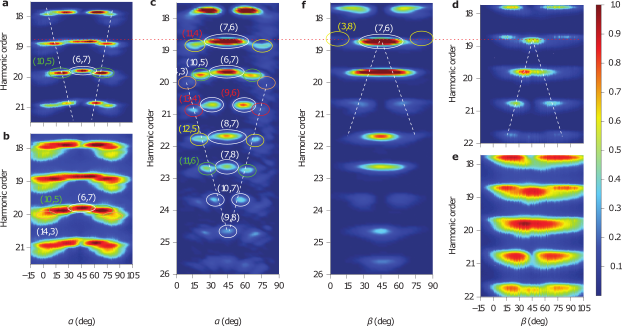
\includegraphics[width=\textwidth]{8-Spin-HHG/Figures/figure8G.png}
  \caption[
  Experimental ellipticity scans on the drivers for bicircular HHG, as observed by A. Fleischer~et~al.
  ]{
  Experimental ellipticity scans for bicircular harmonic generation~\cite{fleischer_spin_2014}, as a function of the waveplate angles $\alpha$ and $\beta$, where $\alpha=\SI{0}{\degree}$ and \SI{90}{\degree} produce a linear fundamental and $\alpha=\SI{45}{\degree}$ makes it circular, and analogously for $\beta$. The spectra are shown in linear~\protect\subref{f8-fleischer-ellipticity-scan-a} and log scale~\protect\subref{f8-fleischer-ellipticity-scan-b}, and in comparison with a linear-scale equivalent TDSE simulation~\protect\subref{f8-fleischer-ellipticity-scan-c} for ellipticity scans of the fundamental, and analogously in \protect\subref{f8-fleischer-ellipticity-scan-d},\,\protect\subref{f8-fleischer-ellipticity-scan-e} and \protect\subref{f8-fleischer-ellipticity-scan-f} for ellipticity scans of the second harmonic.
  Figure excerpted from \citer{fleischer_spin_2014}.
  }
  \label{f8-fleischer-ellipticity-scan}
\end{figure}
\copyrightfootnote{
\reffig{f8-fleischer-ellipticity-scan} copyright tagline.
}



In response to this change in the driving fields, the harmonic emission shows a rich pattern, as exemplified in \reffig{f8-fleischer-ellipticity-scan-a} and the equivalent TDSE simulation in \reffig{f8-fleischer-ellipticity-scan-c}, with the harmonic emission remaining bright over a considerable range of driver ellipticities. Moreover, polarization measurements also revealed that, outside of the bicircular $\alpha=\beta=\SI{45}{\degree}$ centerline the harmonics become elliptically polarized with a range of ellipticities, with the waveplate angles affording significant control over the harmonics' polarization at only moderate cost in the harmonic emission.

The most interesting feature in the experimental spectra is the appearance, out of the centerline, of additional channels that were originally forbidden, and which are very clearly marked by their different redshifts as compared to the integer multiples of the fundamental frequency. Some of these channels appear on the previously forbidden $3k\omega$ harmonics such as the $(9,6)$ channel that is visible in \reffig{f8-fleischer-ellipticity-scan-c} just below $21\omega_1$. Others, like the $(10,5)$ channel below $20\omega_1$, flank the centerline channels after they decay. 


These channels are forbidden in the fully circular case -- there is too much angular momentum for the harmonic photon to take away -- but with the decrease in the angular momentum of the fundamental, they become allowed. However, this viewpoint mostly avoids the real question here: these channels have very evident start and end points over the waveplate angle $\alpha$, and it falls on theory to explain these features. This is unlikely to be possible in a detailed, quantitative way (which can be done via SFA calculations, or even TDSE simulations if necessary, at the cost of an intuitive understanding of the process), but it should be possible to use the quantum theory of spin angular momentum for the light field, at least in an approximate way, to explain the major features of these ellipticity scans.






\section{Conservation of spin angular momentum}

\subsection{Expectation-value model}
\label{sec:expectation-value-model}
In their original work, Fleischer et al. provided a model based on the expectation value of angular momentum, which we will review in this section. It is moderately successful, and provides a reasonable prediction of the existence ranges of several channels, shown as ellipses in \reffig{f8-fleischer-ellipticity-scan}, but it has some conceptual problems and it requires the emission of each individual channel as an open process as regards angular momentum. Later, in section~\ref{sec:decomposition-based-model}, we will propose an alternative model that can also explain the data while retaining the parametric aspect of HHG.


The channel assignments, which are made unambiguous by the detuning of the second harmonic, clearly specify a number of channels at harmonic frequency
\begin{equation}
 \Omega_{(n_1,n_2)}=n_1\omega+n_2 r\omega,
\end{equation}
for integer $n_1$ and $n_2$, and with $r=1.95$, which represent the absorption of $n_1$ fundamental photons and $n_2$ second-harmonic photons. In Fleischer et al.'s expectation-value model, each of these photons is then understood as carrying the expectation value of the spin of its respective field, as is the emitted harmonic photon.


To find this expected value, we take an arbitrary elliptical field with signed ellipticity~$\eps$, and we decompose it as a sum of two opposite circular polarizations, $\ue_R=\tfrac{1}{\sqrt{2}}\left(\ue_x+i\ue_y\right)$ and $\ue_L=\tfrac{1}{\sqrt{2}}\left(\ue_x-i\ue_y\right)$, yielding
\begin{equation}
 \vbf=
 \frac{F_0e^{-i\omega t}}{2\sqrt{2}}
 \left(
 \frac{1+\eps}{\sqrt{1+\eps^2}}\ue_R
 +
  \frac{1-\eps}{\sqrt{1+\eps^2}}\ue_L
 \right)
 +\cc
 \label{e8-elliptical-as-sum-of-circular-polarizations}
\end{equation}
(where we ignore the relative phase between the two components, which gives the orientation of the polarization ellipse). Here the right-circular $\ue_R$ component has definite spin $\sigma_1=+1$ and the left-circular $\ue_L$ has spin $\sigma_2=-1$, which means that the expected spin angular momentum of the field can be calculated to be
\begin{equation}
 \langle\hat{\sigma}\rangle=\frac{2\eps}{1+\eps^2}
 \label{e8-expected-angular-momentum-ellitpicity}
\end{equation}
in units of $\hbar$. For a field generated by shining linearly po\-la\-rized light on a half-wave plate at an angle $\alpha$ to its fast axis, as in the experiment, the ellipticity thus reduces to 
\begin{equation}
 \langle\hat{\sigma}\rangle=\sin(2\alpha).
 \label{e8-expected-angular-momentum-from-angle}
\end{equation}



Under these assumptions, the conservation equation can now be formulated: the spin of the resulting harmonic photon on the channel $(n_1,n_2)$ must be
\begin{equation}
 \langle\hat\sigma_{(n_1,n_2)}\rangle=n_1\langle\hat\sigma_1\rangle + n_2\langle\hat\sigma_2\rangle + \delta_{(n_1,n_2)},
 \label{e8-model-1-equation}
\end{equation}
where $\langle\hat{\sigma}_1\rangle=\sin(2\alpha)$,  $\langle\hat{\sigma}_2\rangle=\sin(2\beta)$, and $\alpha$ and $\beta$ are the angles between the fast axes of the waveplates and the initial linear driver polarizations. 


Here each of the three angular momenta can be measured independently, both experimentally and numerically, and thus a deviation term $\delta_{(n_1,n_2)}$ has been introduced for consistency. Within the expectation-value model, the harmonic generation process is parametric if and only if this term is zero. Fleischer et al. attribute deviations from this to the failure of perturbative nonlinear optics and the presence of additional excitations, and call $\delta_{(n_1,n_2)}$ a `strong field correction'. This model makes multiple predictions which agree with the experiment, though some of them require nonzero values of $\delta_{(n_1,n_2)}$.

\begin{enumerate}[label=(\roman*)]

 \item
 For the symmetric case where $\alpha=\beta=\SI{45}{\degree}$, we have $\sigma_1=1$ and $\sigma_2=-1$, setting \mbox{$\delta_{(n_1,n_2)}=0$} turns the basic relation \eqref{e8-model-1-equation} into $\sigma_{(n_1,n_2)}=n_1-n_2$. From here, imposing the boundedness of photon spins, 
 \begin{equation}
 |\sigma_{(n_1,n_2)}|\leq 1,
 \label{e8-photon-spin-boundedness}
 \end{equation} coupled with the parity constraint, means that $n_1$ and $n_2$ must differ by unity, which matches the experimental predictions.
 
 \item
 As the fundamental driver's waveplate is rotated away from the symmetric case, this restriction must be expanded to include the magnitude of $\sigma_2$, and now reads
 \begin{equation}
 |n_1\sin(2\alpha) - n_2| \leq 1.
 \label{e8-channel-existence-region}
 \end{equation}
 For each channel $n_1$ and $n_2$ are fixed, so this reads as a restriction on $\alpha$, and gives the region where the channel is allowed:
 \begin{equation}
 \frac12\arcsin\left(\frac{n_2-1}{n_1}\right)\leq\alpha\leq\frac12\arcsin\left(\frac{n_2+1}{n_1}\right).
 \label{e8-channel-existence-region-unbundled}
 \end{equation}
 This region matches well the observed range of certain channels, such as (7,6), (8,7), and (9,8), and this provides the basis for the ellipses depicted in \reffig{f8-fleischer-ellipticity-scan}
 
 For certain series of channels, like (13,4), (12,5), (11,6), (10,7) and (9,8), this restriction also correctly predicts a V-shaped pattern where decreasing harmonic order gives an allowed region further from $\alpha=\SI{45}{\degree}$. On the other hand, to obtain the correct regions, correction factors as high as $|\delta_{(n_1,n_2)}|=3$ are required, and these are not consistent across these channels (see, in particular, the supplementary information of \citer{fleischer_spin_2014}).
 
 \item \label{e8-disallowed-channels-discontinuity}
 For certain channels like (6,7) or (7,8), setting $\delta_{(n_1,n_2)}$ to zero makes the restriction~\eqref{e8-channel-existence-region} take the form
 \begin{equation}
 \sin(2\alpha) \geq 1.
 \label{e8-channel-existence-discontinuity}
 \end{equation}
 This implies that parametric channels of this form are only allowed for $\alpha = \SI{45}{\degree}$, but not for any nearby angles. This discontinuity is not present elsewhere in the formalism, and it is not observed in experiment or in simulations, so one is forced, within the expectation-value model, to abandon conservation of spin angular momentum in the generation each individual harmonic.
 
 \item
 In its form $\frac{n_2-1}{n_1}\leq\sin(2\alpha)$, the restriction \eqref{e8-channel-existence-region} means that, for $\beta$ fixed at \SI{45}{\degree}, only channels with $n_1\geq n_2-1$ can exist, which is in agreement with experiment.

\end{enumerate}


Finally, within this model it is possible to study the deviation $\delta_{(n_1,n_2)}$ as a function of the experimental parameters. Fleischer et al. show~\cite{fleischer_spin_2014} that the average of this quantity over all the channels tends to be close to zero, which would indicate the possibility that harmonics are emitted in pairs, with the production of each pair conserving angular momentum. This is indeed possible, in principle, and in such a process Eq.~\eqref{e8-model-1-equation} would be replaced by a more general conservation law for the two correlated channels seen as a single process. However, this picture does require a re-understanding of the three-step model.





\subsection{Decomposition-based model}
\label{sec:decomposition-based-model}

Several of these features of the expectation-value model are undesirable, most markedly the unphysical discontinuity from point \ref{e8-disallowed-channels-discontinuity}, but these can be fixed by going to a slightly more sophisticated model, which we term here the decomposition-based model. This model will allow us to explain the above features while still allowing for the generation of each harmonic to preserve spin angular momentum independently of the other channels.


The key to this model is seeing Eq.~\eqref{e8-elliptical-as-sum-of-circular-polarizations} as indicating the presence of a third wave (a counter-rotating wave at the same, degenerate frequency) which must be included as such, instead of a change to the angular momentum carried by each photon of the driver. To bring this to the forefront, we rephrase expression \eqref{e8-elliptical-as-sum-of-circular-polarizations} in the form
\begin{equation}
 \vbf=
 \frac{F_0e^{-i\omega t}}{2}
 \left(
 \cos(\delta\alpha)\ue_R
 +
  \sin(\delta\alpha)\ue_L
 \right)
 +\cc,
 \label{e8-elliptical-as-two-fields}
\end{equation}
where $\delta\alpha=\alpha-\pi/4$ and we have used $\eps=\tan(\alpha)$. We focus for simplicity on the case where $\beta$ is fixed at \SI{45}{\degree}.


Within the decomposition-based model, the problem consists now of \textit{three} waves which can combine to form harmonics: a left-circular harmonic driver at frequency $r\omega=1.95\omega,$ and two fundamental drivers at frequency $\omega$, one right-circular with relative amplitude $\cos(\delta\alpha)$ and one left-circular with relative amplitude $\sin(\delta\alpha)$. Each channel is now characterized by three integers, $(n_+,n_-;n_2)$, where $n_+$ ($n_-$) photons are absorbed from the right- (left-)circular fundamental driver, and $n_2$ from the harmonic driver, to give an emitted frequency of
\begin{equation}
 \Omega_{(n_+,n_-;n_2)}=(n_+ + n_-)\omega+n_2r\omega.
 \label{e8-model-2-energy-conservation}
\end{equation}


Certain channels require negative values for $n_-$ or $n_+$ for one or both spins of the harmonic photon. In this case, the channel represents stimulated emission into that driver. This is necessary, for example, to explain the observed generation of elliptically polarized photons on channels of the form $(n_1,n_1+1)$ like $(6,7)$ and $(7,8)$. This is, however, not too surprising; in fact, we already met one similar process in \reffig{f8-initial-photon-diagrams-e}. In this extreme nonlinear setting, each harmonic contains contributions from processes of very many orders, and all but the lowest of these contain absorption and stimulated re-emission of photons from and to the driver fields.

Since each field has photons of a definite spin, the conservation of angular momentum reads in this model as
\begin{equation}
 \sigma_{(n_+,n_-;n_2)}=n_+\sigma_+ + n_-\sigma_- + n_2\sigma_2,
 \label{e8-model-2-angular-momentum-conservation}
\end{equation}
where $\sigma_+=+1$ and $\sigma_-=\sigma_2=-1$.


To obtain predictions, we apply the basic principle that the amplitude of an $n$-photon process should scale as the $n^\text{th}$ power of the driving field. This describes the leading term in the corresponding perturbation expansion, and applies both to absorption and to stimulated emission.


As the waveplate is rotated away from the symmetric setting at $\alpha=\SI{45}{\degree}$, the initial energy is transferred from the right-circular driver to the left-circular one. Each channel $(n_+,n_-;n_2)$ absorbs an independent number of photons from each driver, which means that its amplitude must have a basic dependence of the form
\begin{equation}
 F_{(n_+,n_-,n_2)}\sim\cos^{|n_+|}(\delta\alpha)\sin^{|n_-|}(\delta\alpha),
 \label{e8-basic-alpha-dependence}
\end{equation}
and the harmonic intensity is the square of this,
\begin{equation}
 I_{(n_+,n_-;n_2)}\sim\cos^{2|n_+|}(\delta\alpha)\sin^{2|n_-|}(\delta\alpha).
 \label{e8-basic-intensity-alpha-dependence}
\end{equation}
For most channels $n_+$ and $n_-$ are relatively large integers, so the functions in \eqref{e8-basic-alpha-dependence} and \eqref{e8-basic-intensity-alpha-dependence} can be rather sharply peaked. 



Within this model there are no hard boundaries to the existence regions, and the harmonics are in principle possible for any set of laser parameters. Instead, the predictions are in terms for the basic profile of each channel as a function of the driver ellipticity. However, a good approximation to the relevance region of each channel is the region where it is above half of its maximum intensity; we display these regions in \reffig{f8-existence-region-ellipses}. 




\begin{figure}[h]
  \centering
  \subfloat{
    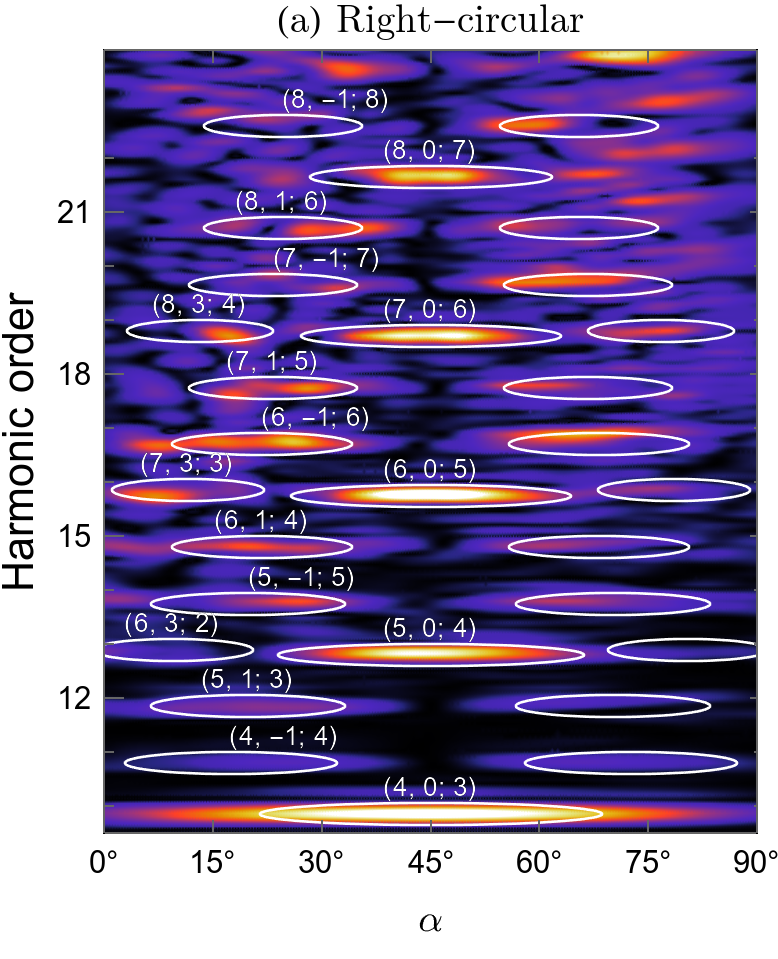
\includegraphics[scale=1]{8-Spin-HHG/Figures/figure8Ia.png}
  }
  \hspace{0mm}
  \subfloat{
    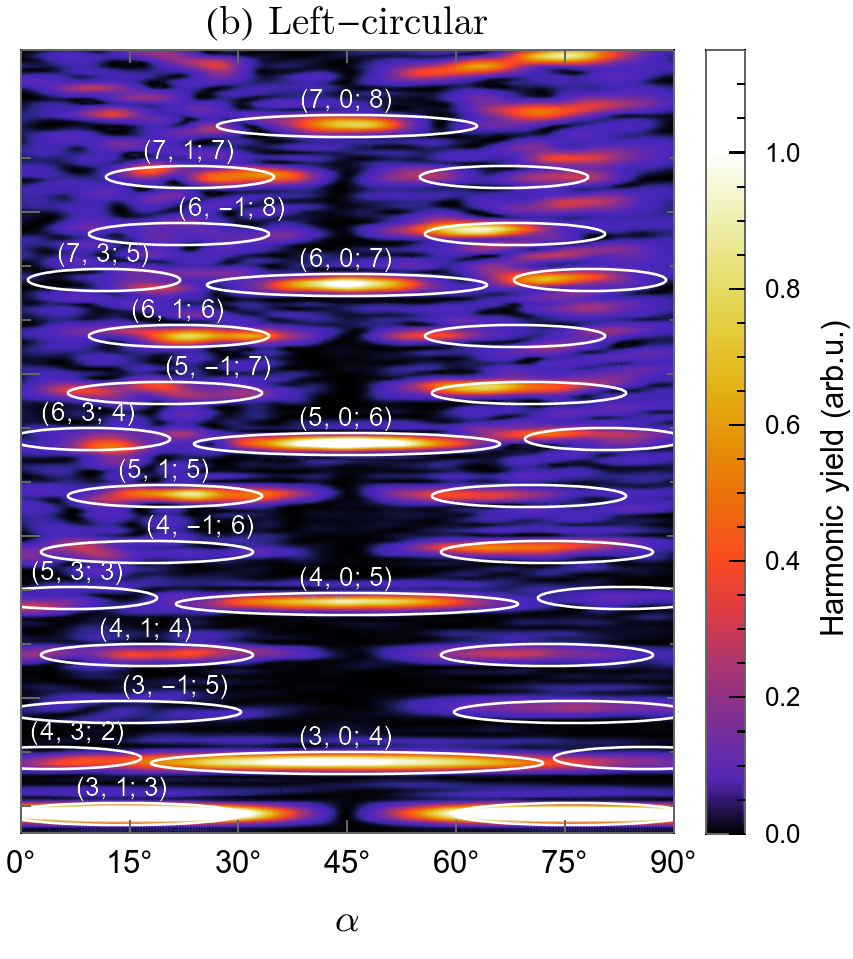
\includegraphics[scale=1]{8-Spin-HHG/Figures/figure8Ib.png}
  }
  
  \captionsetup{width=\textwidth}
  \caption[
  Existence regions for bicircular harmonics using the decomposition-based model, compared to SFA simulations
  ]{
  Existence regions for the different harmonics predicted by the decomposition-based model compared to SFA numerical simulations. The ellipses are drawn with arbitrary widths at the half-maximum-intensity ranges in ellipticity defined by Eq.~\eqref{e8-basic-intensity-alpha-dependence}. We display only the lowest-order channel for each harmonic order and helicity, though higher-order channels are also present which partly overlap with the ones displayed. 
  The simulations use a 10-cycle flat-top envelope with equal-intensity $\SI{2e14}{W/cm^2}$ fields driving argon, as in \citer{fleischer_spin_2014}.
  }
  \label{f8-existence-region-ellipses}
\end{figure}




One interesting feature of this model is that each channel splits into two different channels with opposite spin. For instance, the channel identified as $(10, 5)$ in the expectation-value model, at frequency $\Omega=(10+5r)\omega$, splits into the two channels $(8, 2; 5)$ and $(7, 3; 5)$, with spin $+1$ and $-1$ respectively, giving it an elliptical polarization that depends on the relative weights of the two channels. In general, the channel $(n_1,n_2)$ splits into the \mbox{channels}
\begin{equation}
 (n_+,n_-,n_2)=\left(\frac{n_1+n_2+\sigma}{2},\frac{n_1-n_2-\sigma}{2};n_2\right)
 \label{e8-channel-translation}
\end{equation}
with spin $\sigma=\pm1$. For this expression to give integer $n_\pm$, the sum $n_1+n_2$ must be an odd integer, which matches the parity constraint of the expectation-value model.

As is seen in \reffig{f8-existence-region-ellipses}, the existence regions for these two channels overlap but do not coincide, and they agree rather well with numerical simulations without any free parameters. The superposition of right- and left-circular contributions whose amplitude peaks at different driver ellipticities helps explain the rich dynamics of the polarization of each harmonic shown by both experiment and numerics. 





One important feature of this model is its behaviour for channels of the form $(n_1,0;n_1+1)$, like $(6,0;7)$. As remarked in point \ref{e8-disallowed-channels-discontinuity} above, conservation of angular momentum closes this channel within the expectation-value model for $\alpha\neq\SI{45}{\degree}$: the second-harmonic driver contributes $-7$ units of angular momentum, and the six spins of $\sin(2\alpha)$ are only sufficient to allow a physical harmonic spin of $\sigma \geq -1$ when $\sin(2\alpha)=1$. Within the decomposition-based model, on the other hand, a slightly off-circular field can still produce harmonics: it is seen as a circular field of slightly reduced intensity, with the added presence of a left-circular driver which cannot participate in the process at that order, so the harmonic signal is only reduced slightly, as observed in experiment and in numerics.

The other predictions of the expectation-value model can also be replicated. The symmetric case is identical for both models, so the restriction that $|n_1+n_2|=1$ there also holds; the V-shaped pattern is explained well together with the existence regions of the harmonics; and the restriction that $n_1\geq n_2-1$ is a consequence of the identity $n_+=n_- + n_2 + \sigma$.

It should be stressed, however, that modelling HHG with lowest-order perturbation theory has intrinsic limitations, starting with the complete lack of a harmonic plateau. In this extreme nonlinear setting, many orders of perturbation theory contribute to each harmonic, involving many steps of absorption and stimulated emission of driver photons, and there is as yet no consistent theory to account for their interference. Nevertheless, the basic ellipticity dependence of the lowest order, embodied in \eqref{e8-basic-alpha-dependence} and \eqref{e8-basic-intensity-alpha-dependence}, is a good guide to where to look for each channel; as we have seen, it is remarkably successful.














\section{Subchannel splittings}
\label{sec:subchannel-splittings}
We see, then, that the decomposition-based model can account well for the main features seen in the experiment and in numerical simulations. However, because of its limitations, it is desirable to have additional confirmation that it is indeed the correct way to understand the process.

One way to do this is to exploit the principle that the right- and left-circular components of an elliptical field must be treated independently by actually tuning their frequencies independently. That is, to modify the field in \eqref{e8-elliptical-as-two-fields} into the form
\begin{equation}
 \vbf=
 \frac{E_0}{2}
 \left(
 \cos(\delta\alpha)e^{-i\omega t}\ue_R
 +
  \sin(\delta\alpha)e^{-i\omega' t}\ue_L
 \right)
 +\cc,
 \label{e8-detuned-elliptical-field}
\end{equation}
where the frequency $\omega'$ of the counter-rotating fundamental is now independent of $\omega$. In such a field, the energy conservation equation reads
\begin{equation}
 \Omega_{(n_+,n_-;n_2)}=n_+\omega + n_-\omega'+n_2r\omega,
 \label{e8-modified-energy-conservation}
\end{equation}
and the old channels $(n_1,n_2)$ should split into the two subchannels of \eqref{e8-channel-translation} with a splitting proportional to the detuning $\delta=\omega'-\omega$.



In the time domain, the field in \eqref{e8-detuned-elliptical-field} has an elliptical polarization which slowly rotates over time, since the two circular components, at close to the same frequency, accumulate a relative phase throughout the pulse. Here the axes of this ellipse need to perform at least one full rotation: for a splitting of $\delta$ to be detected in the spectrum, the harmonic linewidth must be of that order, which means the pulse must be longer than $2\pi/\delta$, and therefore the two circular components accumulate a relative phase of at least $2\pi$ over the whole pulse.

This variation on the experiment can, in principle, be tested experimentally, though this adds a further layer of complexity. On the other hand, it is straightforward to implement numerically and it does not add new complications to the numerical methods, which must already be general enough to deal with arbitrary polarizations in two dimensions. (It does, however, add to the required duration of the simulation, which can be a problem for TDSE-based approaches.)






\begin{figure}[b!]
  \centering
  \subfloat{
    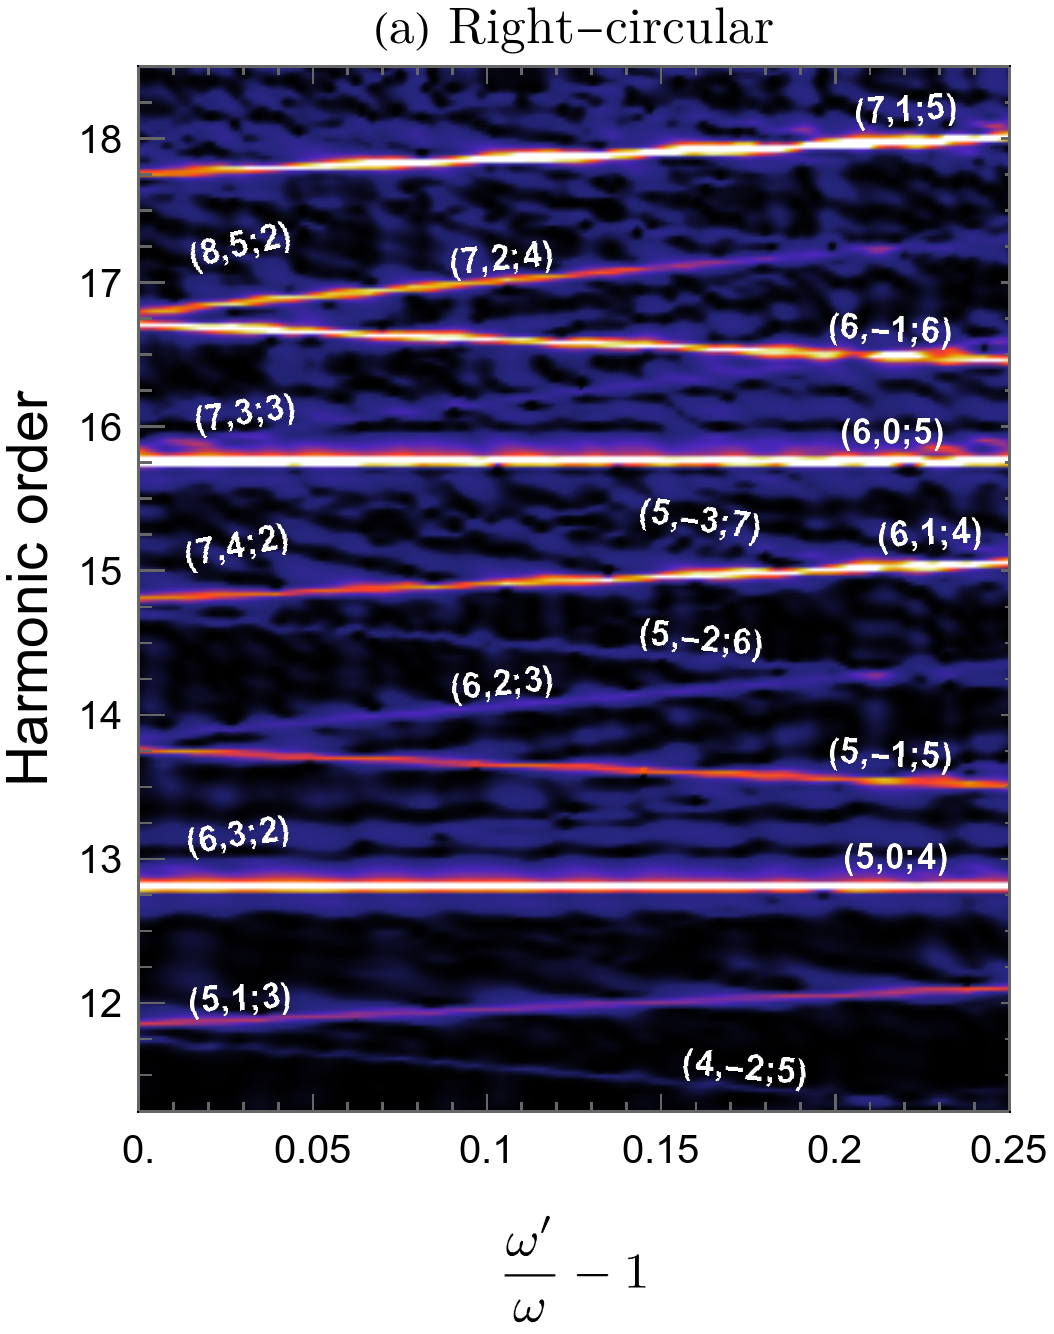
\includegraphics[scale=1]{8-Spin-HHG/Figures/figure8Ja.png}
  }
  \hspace{0mm}
  \subfloat{
    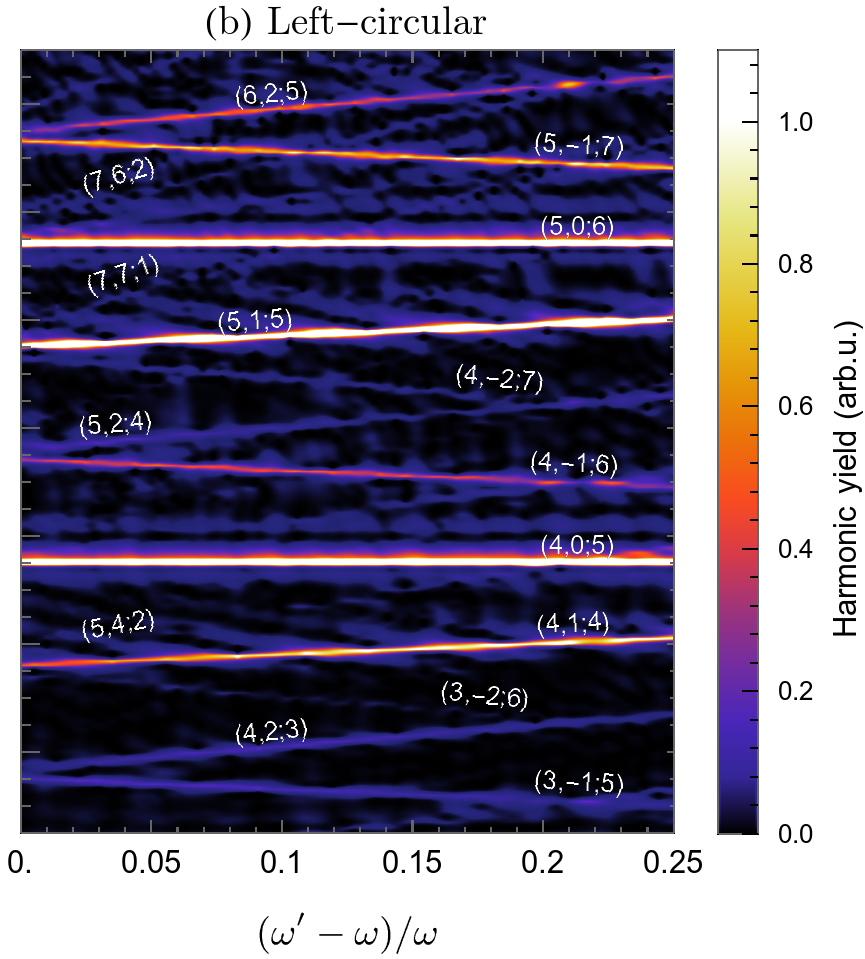
\includegraphics[scale=1]{8-Spin-HHG/Figures/figure8Jb.png}
  }
  
  \captionsetup{width=\textwidth}
  \caption[
  Harmonic spectra for detuned bicircular drivers as a function of the relative detuning $\delta=\omega'/\omega-1$ between the right- and left-circular components of the elliptically polarized fundamental driver
  ]{
  Dependence of the harmonic energies as a function of the relative detuning $\delta/\omega = \omega'/ \omega-1$ between the right- and left-circular components of the elliptically polarized fundamental driver, as in Eq.~\eqref{e8-modified-energy-conservation}, with the different channels marked and changing linearly at different slopes..
  The simulation uses the software from \citer{RB-SFA}, with a 25-cycle flat-top pulse with 2$\tfrac 12$ cycles of sinusoidal on- and off-ramp; we use equal-intensity drivers at $\SI{2e14}{W/cm^2}$, driving argon with an $S$-type orbital, and we set $\alpha=\SI{35}{\degree}$.
  }
  \label{f8-SFA-splittings-spectrum}
\end{figure}


As a test of this variation, then, we calculate the resulting spectra within the SFA, by direct numerical integration as we developed it in \ref{sec:lewenstein-hhg} and as implemented in \citer{RB-SFA}. These results are shown in Fig.~\ref{f8-SFA-splittings-spectrum}, and they show the correct linear dependence of the harmonic energy $\Omega_{(n_+,n_-;n_2)}$ as a function of the relative detuning $\delta/\omega$ between the two circular components of the fundamental. Subchannels with as many as seven photons absorbed from the left-circular component can be identified, even though, at $\alpha=\SI{35}{\degree}$, the counter-rotating component of the fundamental carries only $\sin^2(\delta\alpha)\approx 3\%$ of the total~intensity.





While it is clear that there are additional mechanisms and higher-order channels at work (as shown, particularly, by the intensity modulations of the harmonic lines over detuning), the harmonic energies follow very tightly the essential linear dependence with the correct slopes. This is strong evidence that the photon-exchange picture of the decomposition-based model is the correct way of interpreting the experiment, both in the detuned cases and in the degenerate case of pure elliptical polarization, when $\omega'=\omega$.












%\pagebreak
\section{The four-wave mixing case}
\label{sec:four-wave-mixing}

Having reviewed both models, in the rest of this chapter we will focus on the lowest-order channel, $(1,2)$, which reduces to sum-frequency generation in the standard four-wave mixing nonlinear optics formalism. This process is possible at much lower intensities, where ionized electrons cannot carry away angular momentum, so this brings the problems of the expectation-value model to the fore. This also means that the standard methods of perturbative nonlinear optics are applicable, and we show that this coincides with the predictions of the decomposition-based model.

Consider, then, the channel $(1,2)$, which is of the problematic form $(n_1,n_1+1)$ discussed in point \ref{e8-disallowed-channels-discontinuity} above. This is essentially the generation of the sum frequency $\omega_3=\omega_1+2\omega_2$ \cite{BloembergenSecondHarmonic}, and it can be done at much lower intensities in any medium with an isotropic third-order susceptibility tensor $\chit$; it is shown schematically in \reffig{f8-four-wave-mixing-diagram}. As before, the driver at $\omega_2=r\omega$ is fixed at a left circular polarization, while the ellipticity $\eps$ of the driver at $\omega_1=\omega$ can be varied from right circular through linear to left circular.




\begin{figure}[ht]
  \centering
  
\begingroup
\fontsize{10pt}{12pt}\selectfont

\begin{tikzpicture}[
   scale=0.5,
   level/.style={thick},
   photon/.style={thick,->,shorten >=0.5pt,shorten <=0.5pt,>=stealth},
 ]    
 \nnewlength{\smap} \setlength{\smap}{2.3cm} % small photon
 \nnewlength{\bigp} \setlength{\bigp}{3.6cm} % big photon
 \nnewlength{\offset} \setlength{\offset}{6.3cm} % center of the right and left diagrams
 \nnewlength{\sep} \setlength{\sep}{0.35cm} % (1/2) separation between the up and down arrows of each diagram
 \nnewlength{\lvlwidth} \setlength{\lvlwidth}{0.75cm} % (1/2) width of the horizontal 'level' lines
 \nnewlength{\cancelm} \setlength{\cancelm}{0.82cm} % horizontal offset of the center of the cancelling cross
 \nnewlength{\canceld} \setlength{\canceld}{0.75cm} % (1/2) horizontal width of the cancelling cross
 \nnewlength{\cancelv} \setlength{\cancelv}{1.7cm} % (1/2) height of the cancelling cross
%
 \draw[level] (-\offset-\lvlwidth,  0cm) -- (-\offset+\lvlwidth,  0cm);
 \draw[level] (-\offset-\lvlwidth,\smap+2\bigp) -- (-\offset+\lvlwidth,\smap+2\bigp);
 \draw[photon] (-\offset-\sep,    0cm) -- (-\offset-\sep, \smap) node[midway, left] {\begin{turn}{90}$\omega_1,\,\eps$\epol\end{turn}};
 \draw[photon] (-\offset-\sep,  \smap) -- (-\offset-\sep,\smap+\bigp) node[midway, left] {\begin{turn}{90}$\omega_2,\leftpol$\end{turn}};
 \draw[photon] (-\offset-\sep, \smap+\bigp) -- (-\offset-\sep,\smap+2\bigp) node[midway, left] {
    \begin{turn}{90}$\omega_2,\leftpol$ \end{turn}
    };
 \draw[photon] (-\offset+\sep,\smap+2\bigp) -- (-\offset+\sep,  0cm) node[midway,right] {\begin{turn}{90}$\omega_1+ 2\omega_2,$ ?\end{turn}};
%
 \node at (-\offset/2-1.2cm,\smap/2+\bigp-0.08cm) {\scalebox{1.5}{$=$}};
 \node at (-\offset/2+0.5cm,\smap/2+\bigp) {$\cos(\delta\alpha)$};
%
 \draw[level] (-\lvlwidth,  0cm) -- (\lvlwidth,  0cm);
 \draw[level] (-\lvlwidth,\smap+2\bigp) -- (\lvlwidth,\smap+2\bigp);
 \draw[photon] (-\sep,    0cm) -- (-\sep, \smap) node[midway, left] {\begin{turn}{90}$\omega_1,\rightpol$\end{turn}};
 \draw[photon] (-\sep,  \smap) -- (-\sep,\smap+\bigp) node[midway, left] {\begin{turn}{90}$\omega_2,\leftpol$\end{turn}};
 \draw[photon] (-\sep, \smap+\bigp) -- (-\sep,\smap+2\bigp) node[midway, left] {\begin{turn}{90}$\omega_2,\leftpol$ \end{turn}};
 \draw[photon] (\sep,\smap+2\bigp) -- (\sep,  0cm) node[midway,right] {\begin{turn}{90}$\omega_1+ 2\omega_2,\leftpol$\end{turn}};
%
 \node at (\offset/2-1.0cm,\smap/2+\bigp-0.006cm) {\scalebox{1.5}{$+$}};
 \node at (\offset/2+0.65cm,\smap/2+\bigp) {$\sin(\delta\alpha)$};
%
 \draw[level] (\offset-\lvlwidth,  0cm) -- (\offset+\lvlwidth,  0cm);
 \draw[level] (\offset-\lvlwidth,\smap+2\bigp) -- (\offset+\lvlwidth,\smap+2\bigp);
 \draw[photon] (\offset-\sep,    0cm) -- (\offset-\sep, \smap) node[midway, left] {\begin{turn}{90}$\omega_1,\leftpol$\end{turn}};
 \draw[photon] (\offset-\sep,  \smap) -- (\offset-\sep,\smap+\bigp) node[midway, left] {\begin{turn}{90}$\omega_2,\leftpol$\end{turn}};
 \draw[photon] (\offset-\sep, \smap+\bigp) -- (\offset-\sep,\smap+2\bigp) node[midway, left] {\begin{turn}{90}$\omega_2,\leftpol$\end{turn}};
 \draw[photon] (\offset+\sep,\smap+2\bigp) -- (\offset+\sep,  0cm) node[midway,right] {\begin{turn}{90}$\omega_1+ 2\omega_2, \,3\!\leftpol$\end{turn}};
%
 \draw[thick] (\offset+\cancelm - \canceld, \smap/2+\bigp - \cancelv) -- (\offset+\cancelm + \canceld, \smap/2+\bigp + \cancelv);
 \draw[thick] (\offset+\cancelm + \canceld, \smap/2+\bigp - \cancelv) -- (\offset+\cancelm - \canceld, \smap/2+\bigp + \cancelv);
%
\end{tikzpicture}

\endgroup










  
  \vspace{3mm}
  \caption[
  Feynman diagram for the $(1,2)$ channel in bicircular HHG with one elliptical and one circular driver
  ]{
  The channel $(1,2)$, essentially a four-wave mixing process at its lowest order and therefore also observable in the perturbative regime, for an elliptical driver at frequency $\omega_1$ and a left-circular driver at frequency $\omega_2$ combining to make a left-circular harmonic at frequency $\omega_1+\omega_2$. By decomposing the elliptical driver as a superposition of circular polarizations one obtains an allowed process with a right-circular $\omega_2$ driver, and a forbidden process with three left-circular drivers which has too much angular momentum for a single harmonic photon.
  }
\label{f8-four-wave-mixing-diagram}
\end{figure}






From the perspective of the expectation-value model, the process cannot happen unless the $\omega_1$ driver has a right circular polarization, with an ellipticity of $\eps=1$. If the field is even slightly elliptical, the expectation value of the spin per photon decreases to $\langle\sigma_1\rangle  =2\eps/(1+\eps^2) =\sin(2\alpha) <1$, and there is no longer a way for the total spin to be greater than~$-1$.

Within the decomposition-based model, on the other hand, the elliptical driver is understood as a superposition of circularly polarized drivers of spin $\pm1$, each with amplitude $(1\pm\eps)/\sqrt{2(1+\eps^2)}$. If the polarization is slightly off-circular, most of the amplitude is in the right-circular driver, which can still participate in the process, and a slightly reduced harmonic signal is obtained. 

$\quad$

More specifically, as the allowed process takes in one photon from the right-circular component at frequency $\omega_1$, the harmonic field will be proportional to the component's amplitude,
\begin{equation}
E\sim\frac{1+\eps}{\sqrt{2(1+\eps^2)}}=\cos(\delta\alpha),
\end{equation}
and the output intensity will be the square of this. Here one should also note that there will be some nonzero harmonic intensity for \textit{all} ellipticities except for the completely left-circular case, which includes many cases with negative expectation value of the \mbox{photon spin}.



The predictions of the decomposition-based model are here in complete agreement with the predictions of standard perturbative nonlinear optics \cite{VectorFourWaveMixing, AgrawalFiberOptics}, which was shown early on to conserve spin angular momentum \cite{BloembergenConservationLaws, SelectionRulesNonlinearOptics}. In this treatment, the sum-frequency wave at $\omega_3=\omega_1+2\omega_2$ is generated by the nonlinear polarization 
\begin{equation}
\vbP^{(3)}=\epsilon_0\chit
\tdots
\vbf\,\vbf\,\vbf,
\label{e8-nonlinear-polarization-definition}
\end{equation}
where the vertical dots denote a three-way tensor contraction. In component form, this relation reads $P^{(3)}_i=\epsilon_0 \sum_{jkl} \chi^{(3)}_{ijkl} F_jF_kF_l$.



To obtain the sum-frequency component of this polarization, one expresses the electric field as a sum over the participating modes, 
\begin{equation}
  \vbf=\sum_{\alpha=1}^3\left[
  \vbf_\alpha e^{i(\vbk_\alpha\cdot \vbr-\omega_\alpha t)}
  +
  \vbf_\alpha^\ast e^{-i(\vbk_\alpha\cdot \vbr-\omega_\alpha t)}
  \right]
  \label{e8-electric-field-with-conjugate}
\end{equation}
and looks for the component of the polarization which oscillates as $e^{i(\vbk_3\cdot\vbr-\omega_3 t)}$. Substituting the expression~\eqref{e8-electric-field-with-conjugate} into the contraction in \eqref{e8-nonlinear-polarization-definition} results in eight terms, depending on whether $\vbf_\alpha$ or its conjugate is taken. Each of the eight terms describes a different process, which include parametric amplification or self- and cross-phase modulation \cite{AgrawalFiberOptics}; the sum-frequency generation process we want is the term with three factors of  $\vbf_\alpha$. This has the polarization amplitude
\begin{equation}
\vbP_3=\epsilon_0\chit
\tdots
\vbf_1\vbf_2\vbf_2 e^{i\varphi},
\label{e8-nonlinear-polarization-amplitudes}
\end{equation}
where $\varphi=(\vbk_1+2\vbk_2-\vbk_3)\cdot\vbr-(\omega_1+2\omega_2-\omega_3)t$.




To calculate the contraction in \eqref{e8-nonlinear-polarization-amplitudes} we impose the isotropy condition on the susceptibility tensor $\chit$. The only isotropic tensors of rank 4 have a component form $\delta_{ij}\delta_{kl}$ \cite[\S3.03]{JeffreysJeffreys}, which corresponds to the tensor action 
\begin{equation}
\stackrel{\leftrightarrow}{\delta}\, \,\tdots\vb{u}\vb{v}\vb{w}=\vb{u}(\vb{v}\cdot\vb{w}).
\end{equation}
That is, the tensor contracts its second and third inputs, and produces a vector along its first input. The contraction in \eqref{e8-nonlinear-polarization-amplitudes} produces three terms of this form, with different permutations of its inputs. Each of these terms will in principle have a different frequency-dependent complex scalar susceptibility $\chi^{(3)}_\text{s}(\omega_\alpha,\omega_\beta,\omega_\gamma)$, but only one term will be allowed so this distinction can be dropped.





Under these conditions, the sum-frequency polarization becomes
%\vspace{-1mm} %% to prevent some horrible spacings between text and equations. HACK!
\begin{equation}
\vbP_3=\epsilon_0\chis e^{i\varphi} \left(\vphantom{\sum_i}
2\vbf_2(\vbf_1\cdot\vbf_2)+\vbf_1(\vbf_2\cdot\vbf_2)
\right).
\label{e8-nonlinear-polarization-inner-products}
\end{equation}
Here $\vbf_2=F_2\ue_L$ is left polarized, which means that the second term vanishes: in a frame where the propagation direction is in the $z$ axis,
\begin{equation}
 \ue_L\cdot\ue_L=
 \frac{1}{\sqrt{2}}\begin{pmatrix}1\\i\\0\end{pmatrix}
 \cdot
 \frac{1}{\sqrt{2}}\begin{pmatrix}1\\i\\0\end{pmatrix}
 =0.
\label{e8-el-dot-el-inner-product}
\end{equation}
The amplitude for the field at $\omega_1$ encodes the ellipticity dependence, through the analog of~\eqref{e8-elliptical-as-sum-of-circular-polarizations},
\begin{equation}
 \vbf_1=
 F_1
 \left(
 \frac{1+\eps}{\sqrt{2(1+\eps^2)}}\ue_R
 +
  \frac{1-\eps}{\sqrt{2(1+\eps^2)}}\ue_L
 \right).
 \label{e8-elliptical-driver-polarization-decomposition}
\end{equation}
This is projected on the amplitude $\vbf_2$, which eliminates the left-circular component as per the inner product in~\eqref{e8-el-dot-el-inner-product}, and multiplies the left-circular vector $\vbf_2$, so that the final amplitude is
\begin{equation}
\vbP_3=\epsilon_0\chis e^{i\varphi} F_1F_2^2 \frac{1+\eps}{\sqrt{2(1+\eps^2)}}\ue_L.
\label{e8-nonlinear-polarization-final-result}
\end{equation}





The ellipticity dependence of this result is exactly that predicted by the decomposition-based model, and indeed it's clear that its predictions in the general case simply represent the leading-order perturbative term for the channel; the expectation-value model, on the other hand, predicts the process is forbidden except for $\eps=1$. Therefore, at least in the cases where perturbative optics holds, using the expectation value of each photon's angular momentum in the conservation equation leads to incorrect results. 

This is slightly counter-intuitive, as one does expect a conservation equation to hold at the level of expectation values for every conserved quantity, but a direct application in the form of Eq.~\eqref{e8-model-1-equation} is inconsistent with formal perturbative treatments where those are available, and would need further justification for its use in more highly nonlinear cases.

Nevertheless, it is indeed possible to understand the generation of harmonics by elliptical drivers, in both the perturbative and extreme-nonlinear cases, in terms of a simple photon picture, even when that photon picture is manifestly inadequate for many essential aspects of the emitted radiation. Our model provides a simple framework for this understanding, which is in agreement with the available experimental observations and whose predictions are borne out by numerical calculations. 

This allows us to conclude, then, that high-order harmonic generation generally conserves spin angular momentum, in the detailed sense of parametric photon-to-photon processes -- or, at least, it does so in this specific situation, which stretches that behaviour to its limits. HHG, as shown in our model and later minor extensions by others~\cite{milosevic_bicircular-angular-momentum_2015}, is so far consistent with a picture as a parametric process where multiple driver photons get up-converted into harmonic photons and the atom returns to its ground state after the recombination step, at least as far as angular momentum is conserved.



































%\begin{figure}[t!]
%  \centering
%  \subfloat{\label{f8-fleischer-ellipticity-results-a}}
%  \subfloat{\label{f8-fleischer-ellipticity-results-b}}
%  \subfloat{\label{f8-fleischer-ellipticity-results-c}}
%  \subfloat{\label{f8-fleischer-ellipticity-results-d}}
%  \subfloat{\label{f8-fleischer-ellipticity-results-e}}
%  \subfloat{\label{f8-fleischer-ellipticity-results-f}}
%  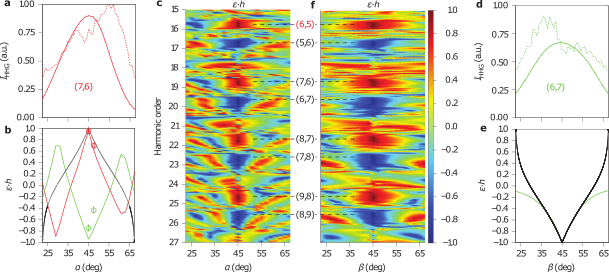
\includegraphics[width=\textwidth]{8-Spin-HHG/Figures/figure8H.png}
%  \caption{
%  Ellipticity measurements for bicircular harmonic 
%  Figure excerpted from \citer{fleischer_spin_2014}.
%  }
%  \label{f8-fleischer-ellipticity-results}
%\end{figure}
%\unmarkedfntext{
%\reffig{f8-fleischer-ellipticity-results} copyright tagline.
%}








%\vspace{1.5cm}
%
%
%Experiment. Fleischer original \cite{fleischer_spin_2014}. Then brighter and with XMCD in \cite{kfir_generation_2015, fan_bright-circularly_2015}, mix of 800+1300 in \cite{fan_bright-circularly_2015}, chiral phase matching \cite{kfir_chiral-phase-matching_2016}, in-line generation \cite{kfir_in-line-bicircular_2016}. Noncollinear \cite{hickstein_non-collinear_2015}.
%
%
%Initial theory \cite{EichmannExperiment, SFALong, SFAMilosevic, milosevic_bicircular-hhg_2000, SFAMilosevicBecker, milosevic_unusual-nonlinear-polarization_2000, milosevic_hhg-laser-phys_2001, averbukh_stability_2002, SFACeccherini, MilosevicIsolatedPulses},
%
%First full quantum-orbit \cite{SFAMilosevicBecker}. First time-dependent view of APT \cite{milosevic_unusual-nonlinear-polarization_2000}.
%
%
%Elliptical fields kill HHG, \cite{moller_hhg-elliptical-fields_2012}, but it's actually just down to selection rules \cite{SelectionRulesInHHG}.
%
%
%Theory after the Fleischer expt: 
%\cite{milosevic_bicircular-angular-momentum_2015} \cite{milosevic_circularly_2015}  \cite{medisauskas_generating_2016} \cite{hernandez_isolated-circular-pulses_2016} 
%\cite{reich-madsen_rotating-frame-bicircular_2016, reich-madsen_molecular-symmetries_2016} %the latter with detuning plots similar to mine
%\cite{baykusheva_bicircular-hhg-spectroscopy}, \cite{liu_selection-rules-hhg_2016}, \cite{mauger_bicircular-molecular-hhg}, \cite{odzak_polyatomic-bicircular_2016} \cite{yuan-bandrauk_circular-hhg-extended-asymmetric-molecules_2011}
%
%Detuning plots in \cite{reich-madsen_molecular-symmetries_2016}
%
%
%
%Circular attosecond pulses in \cite{medisauskas_generating_2016, hernandez_isolated-circular-pulses_2016}
%
%
%
%Ionization in bicircular fields \cite{mancuso_bicircular-ionization_2015,mancuso_bicircular-rescattering_2016,ngoko-starace_multistart-spiral-ionization_2016, milosevic_bicircular-ionization-sfa_2016, eckart_bicircular-nsdi_2016, chaloupka_bicircular-double-ionization_2016, kramo_bicircular-atd_2007}
%
%Laser-assisted recombination \cite{odzak_bicircular-laser-assisted-recombination_2015}
%
%Electron rescattering \cite{hasovic_rescattering-bicircular_2016}
%
%Elliptical APTs from $p$ states \cite{milosevic_elliptical-apt_2015}		
%
%Using it for spin polarization \cite{milosevic_bicircular-spin-polarization_2016, hartung_spin-polarization-ionization_2016}
%
%
%Polarimetry \cite{veyrinhas_polarimetry-original_2013, veyrinhas_depolarized-hhg-atto_2015}, \cite{chen_tomographic-hhg-polarimetry_2016}
%
%\def\bibAnnoteFile#1{\texttt{\detokenize{#1}}}
%\setlist{noitemsep}
%
%Circular harmonics experiments:
%\begin{itemize}
%  \item Ferré, elliptical driver, resonant harmonics \cite{ferre_circular-harmonics_2015}
%  \item Vodungbo XUV waveplate \cite{vodungbo_hhg-waveplate_2011}, single application in \cite{willems_hhg-waveplate_2015}.
%  \item linear driver with aligned molecules  \cite{zhou_aligned-molecules-elliptical-hhg_2009}
%  \item Circular XUV from FELs \cite{bahrdt_fel-circular-initial_1992} \cite{allaria_FEL-circular_2014} \cite{lutman_FEL-polarization_2016}
%  \item plasma-based soft-X-ray laser \cite{depresseux_hhg-then-plasma-laser_2015},  built on top of Vodungbo waveplate
%\end{itemize}
%
%Circular harmonics proposals:
%\begin{itemize}
%  \item via quasi phase matching \cite{liu_circular-hhg-quasi-phase-matching_2012}
%  \item crossed beams, linear plus elliptical in the orthogonal plane \cite{fleischer_linear-plus-elliptical-driver_2013}
%  \item cross-polarized two colour \cite{lambert_circular-hhg-cross-polarized_2015}, \cite{ruiz_elliptical-pulses-two-color_2009}
%\end{itemize}







































